%% abtex2-modelo-trabalho-academico.tex, v-1.9.6 laurocesar
%% Copyright 2012-2016 by abnTeX2 group at http://www.abntex.net.br/
%%
%% This work may be distributed and/or modified under the
%% conditions of the LaTeX Project Public License, either version 1.3
%% of this license or (at your option) any later version.
%% The latest version of this license is in
%%   http://www.latex-project.org/lppl.txt
%% and version 1.3 or later is part of all distributions of LaTeX
%% version 2005/12/01 or later.
%%
%% This work has the LPPL maintenance status `maintained'.
%%
%% The Current Maintainer of this work is the abnTeX2 team, led
%% by Lauro César Araujo. Further information are available on
%% http://www.abntex.net.br/
%%
%% This work consists of the files abntex2-modelo-trabalho-academico.tex,
%% abntex2-modelo-include-comandos and abntex2-modelo-references.bib
%%

% ------------------------------------------------------------------------
% ------------------------------------------------------------------------
% abnTeX2: Modelo de Trabalho Academico (tese de doutorado, dissertacao de
% mestrado e trabalhos monograficos em geral) em conformidade com
% ABNT NBR 14724:2011: Informacao e documentacao - Trabalhos academicos -
% Apresentacao
% ------------------------------------------------------------------------
% ------------------------------------------------------------------------

\documentclass[
	% -- opções da classe memoir --
	12pt,				% tamanho da fonte
	openright,			% capítulos começam em pág ímpar (insere página vazia caso preciso)
	oneside,			% para impressão em recto e verso. Oposto a oneside
	a4paper,			% tamanho do papel.
    sumario=tradicional, % modelo de sumário
	% -- opções da classe abntex2 --
	%chapter=TITLE,		% títulos de capítulos convertidos em letras maiúsculas
	%section=TITLE,		% títulos de seções convertidos em letras maiúsculas
	%subsection=TITLE,	% títulos de subseções convertidos em letras maiúsculas
	%subsubsection=TITLE,% títulos de subsubseções convertidos em letras maiúsculas
	% -- opções do pacote babel --
	english,			% idioma adicional para hifenização
	french,				% idioma adicional para hifenização
	spanish,			% idioma adicional para hifenização
	brazil				% o último idioma é o principal do documento
	]{ppgec-abntex2}

% ---
% Pacotes básicos
% ---
\usepackage{times}			    % Usa a fonte Times New Roman
\usepackage[T1]{fontenc}		% Selecao de codigos de fonte.
\usepackage[utf8]{inputenc}		% Codificacao do documento (conversão automática dos acentos)
\usepackage{lastpage}			% Usado pela Ficha catalográfica
\usepackage{indentfirst}		% Indenta o primeiro parágrafo de cada seção.
\usepackage{color}				% Controle das cores
\usepackage{graphicx}			% Inclusão de gráficos
\usepackage{microtype} 			% para melhorias de justificação
% ---

% ---
% Pacotes adicionais, usados apenas no âmbito do Modelo Canônico do abnteX2
% ---
\usepackage{lipsum}				% para geração de dummy text
% ---

% ---
% Pacotes customizados
% ---
\usepackage{algorithm}
\floatname{algorithm}{Algoritmo}
\usepackage[noend]{algpseudocode}
\usepackage{multirow}
%\usepackage[portugues,ruled,lined]{algorithm2e}
%\usepackage{algorithmic}

% ---
% Pacotes de citações
% ---
\usepackage[num,abnt-etal-list=0]{abntex2cite}	% Citações padrão ABNT, removendo et al na bibliografia
\citebrackets[]
% hack para colocar colchetes nas referencias.
\makeatletter
\ifthenelse{\boolean{ABCIbiblabelonmargin}}
{
\renewcommand{\@biblabel}[1]%
{\ifthenelse{\equal{#1}{}}{}{{\citenumstyle #1\hspace{\biblabelsep}}}}
}
{
\renewcommand{\@biblabel}[1]%
{%
\ifthenelse{\equal{#1}{}}
{}
{%
\def\biblabeltext{{\citenumstyle [#1]\hspace{\biblabelsep}}}%
\settowidth{\ABCIauxlen}{\biblabeltext}%
\ifthenelse{\lengthtest{\ABCIauxlen<\minimumbiblabelwidth}}
{\setlength{\ABCIauxlen}{\minimumbiblabelwidth-\ABCIauxlen}}
{\setlength{\ABCIauxlen}{0cm}}%
{\biblabeltext\hspace{\ABCIauxlen}}%
}%
}%
}
\makeatother
% ---
% Informações de dados para CAPA e FOLHA DE ROSTO
% ---
% ---
% Informações de dados para CAPA e FOLHA DE ROSTO
% ---

\titulo{Otimizando o Team Ant Colony System \\para cálculo de múltiplas rotas para a distribuição de materiais e medicamentos}
\autor{Renan Costa Alencar}
\local{Recife}
\data{outubro de 2018}
\orientador{Prof. DSc. Carmelo José Albanez Bastos Filho}
\coorientador{}
\instituicao{
  \SingleSpacing
  Universidade de Pernambuco \\
  Escola Politécnica de Pernambuco \\
  Programa de Pós-Graduação Acadêmica em Engenharia de Computação
}
\tipotrabalho{Dissertação de Mestrado}
% O preambulo deve conter o tipo do trabalho, o objetivo,
% o nome da instituição e a área de concentração
\preambulo{Dissertação apresentada ao Programa de Pós-Graduação acadêmico em ENGENHARIA DE COMPUTAÇÃO da Universidade de Pernambuco como requisito parcial para obtenção do título de Mestre em Engenharia de Computação.}
% ---



% ---
% Configurações de aparência do PDF final

% alterando o aspecto da cor azul
\definecolor{blue}{RGB}{41,5,195}

% informações do PDF
\makeatletter
\hypersetup{
     	%pagebackref=true,
		pdftitle={\@title},
		pdfauthor={\@author},
    	pdfsubject={\imprimirpreambulo},
	    pdfcreator={LaTeX with abnTeX2},
		pdfkeywords={abnt}{latex}{abntex}{abntex2}{trabalho acadêmico},
		colorlinks=true,       		% false: boxed links; true: colored links
    	linkcolor=blue,          	% color of internal links
    	citecolor=blue,        		% color of links to bibliography
    	filecolor=magenta,      		% color of file links
		urlcolor=blue,
		bookmarksdepth=4
}
\makeatother
% ---

% ---
% Espaçamentos entre linhas e parágrafos
% ---

% O tamanho do parágrafo é dado por:
\setlength{\parindent}{1.3cm}

% Controle do espaçamento entre um parágrafo e outro:
\setlength{\parskip}{0.2cm}  % tente também \onelineskip

% ---
% compila o indice
% ---
\makeindex
% ---

%%% -----
%%% Formato de cabeçalho/rodapé romano nos elementos pré-textuais
%%% -----

%% Novo estilo
\makepagestyle{estilo_pretextual} %%% escolha um nome
\makeevenhead{estilo_pretextual}{}{}{\ABNTEXfontereduzida \textit \thepage}
\makeoddhead{estilo_pretextual}{}{}{\ABNTEXfontereduzida \textit \thepage}

%% Customiza comando \pretextual
\renewcommand{\pretextual}{

  \aliaspagestyle{chapter}{estilo_pretextual}% customizing chapter pagestyle
  \pagestyle{estilo_pretextual}
  \aliaspagestyle{cleared}{empty}
  \aliaspagestyle{part}{estilo_pretextual}
}

% ---
% Ajusta a marca \textual para que a numeração volte a ser arábica
% nos elementos textuais
\let\oldtextual\textual        % copia o comando \textual anterior para \oldtextual
\renewcommand{\textual}{%
  \oldtextual%
  \pagenumbering{arabic} % volta à numeração arábica
}
% ---



% ----
% Início do documento
% ----
\begin{document}

% Seleciona o idioma do documento (conforme pacotes do babel)
%\selectlanguage{english}
\selectlanguage{brazil}

% Retira espaço extra obsoleto entre as frases.
\frenchspacing

% ----------------------------------------------------------
% ELEMENTOS PRÉ-TEXTUAIS
% ----------------------------------------------------------


% ---
% Capa
% ---
\imprimircapa
% ---

% ---
% Folha de rosto
% (o * indica que haverá a ficha bibliográfica)
% ---
\thispagestyle{empty}
\imprimirfolhaderosto*
% ---

% Inicia a numeração dos elementos pre textuais após a folha de rosto
\pagenumbering{roman} %%% ou \pagenumbering{Roman}

% ---
% Inserir a ficha bibliografica
% ---

% Porém, a biblioteca da sua lhe fornecerá um PDF
% com a ficha catalográfica definitiva após a defesa do trabalho. Quando estiver
% com o documento, salve-o como PDF no diretório do seu projeto e substitua todo
% o conteúdo de implementação deste arquivo pelo comando abaixo:
%
% \begin{fichacatalografica}
%     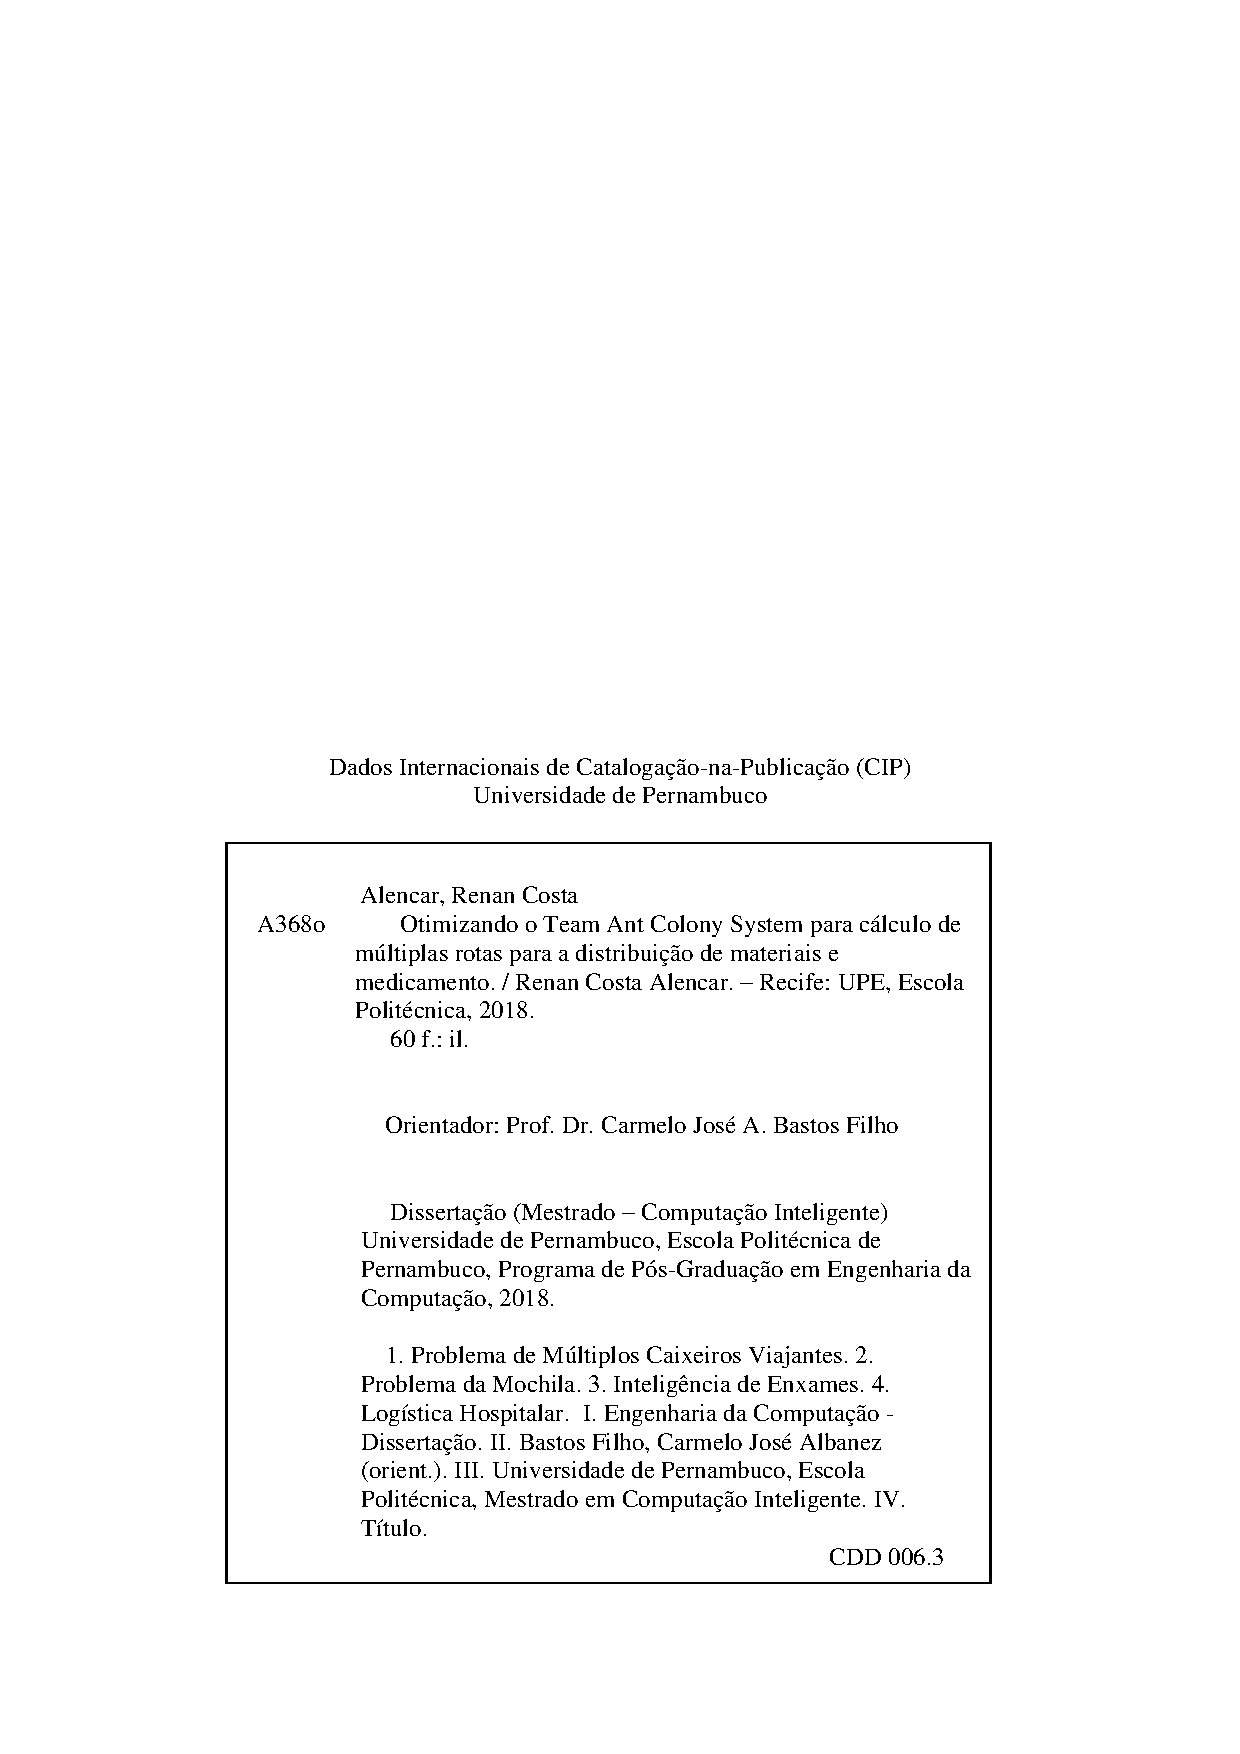
\includepdf{fig_ficha_catalografica.pdf}
% \end{fichacatalografica}

% ---

% ---
% Inserir folha de aprovação
% ---

% Isto é um exemplo de Folha de aprovação, elemento obrigatório da NBR
% 14724/2011 (seção 4.2.1.3). Você pode utilizar este modelo até a aprovação
% do trabalho. Após isso, substitua todo o conteúdo deste arquivo por uma
% imagem da página assinada pela banca com o comando abaixo:
%
% 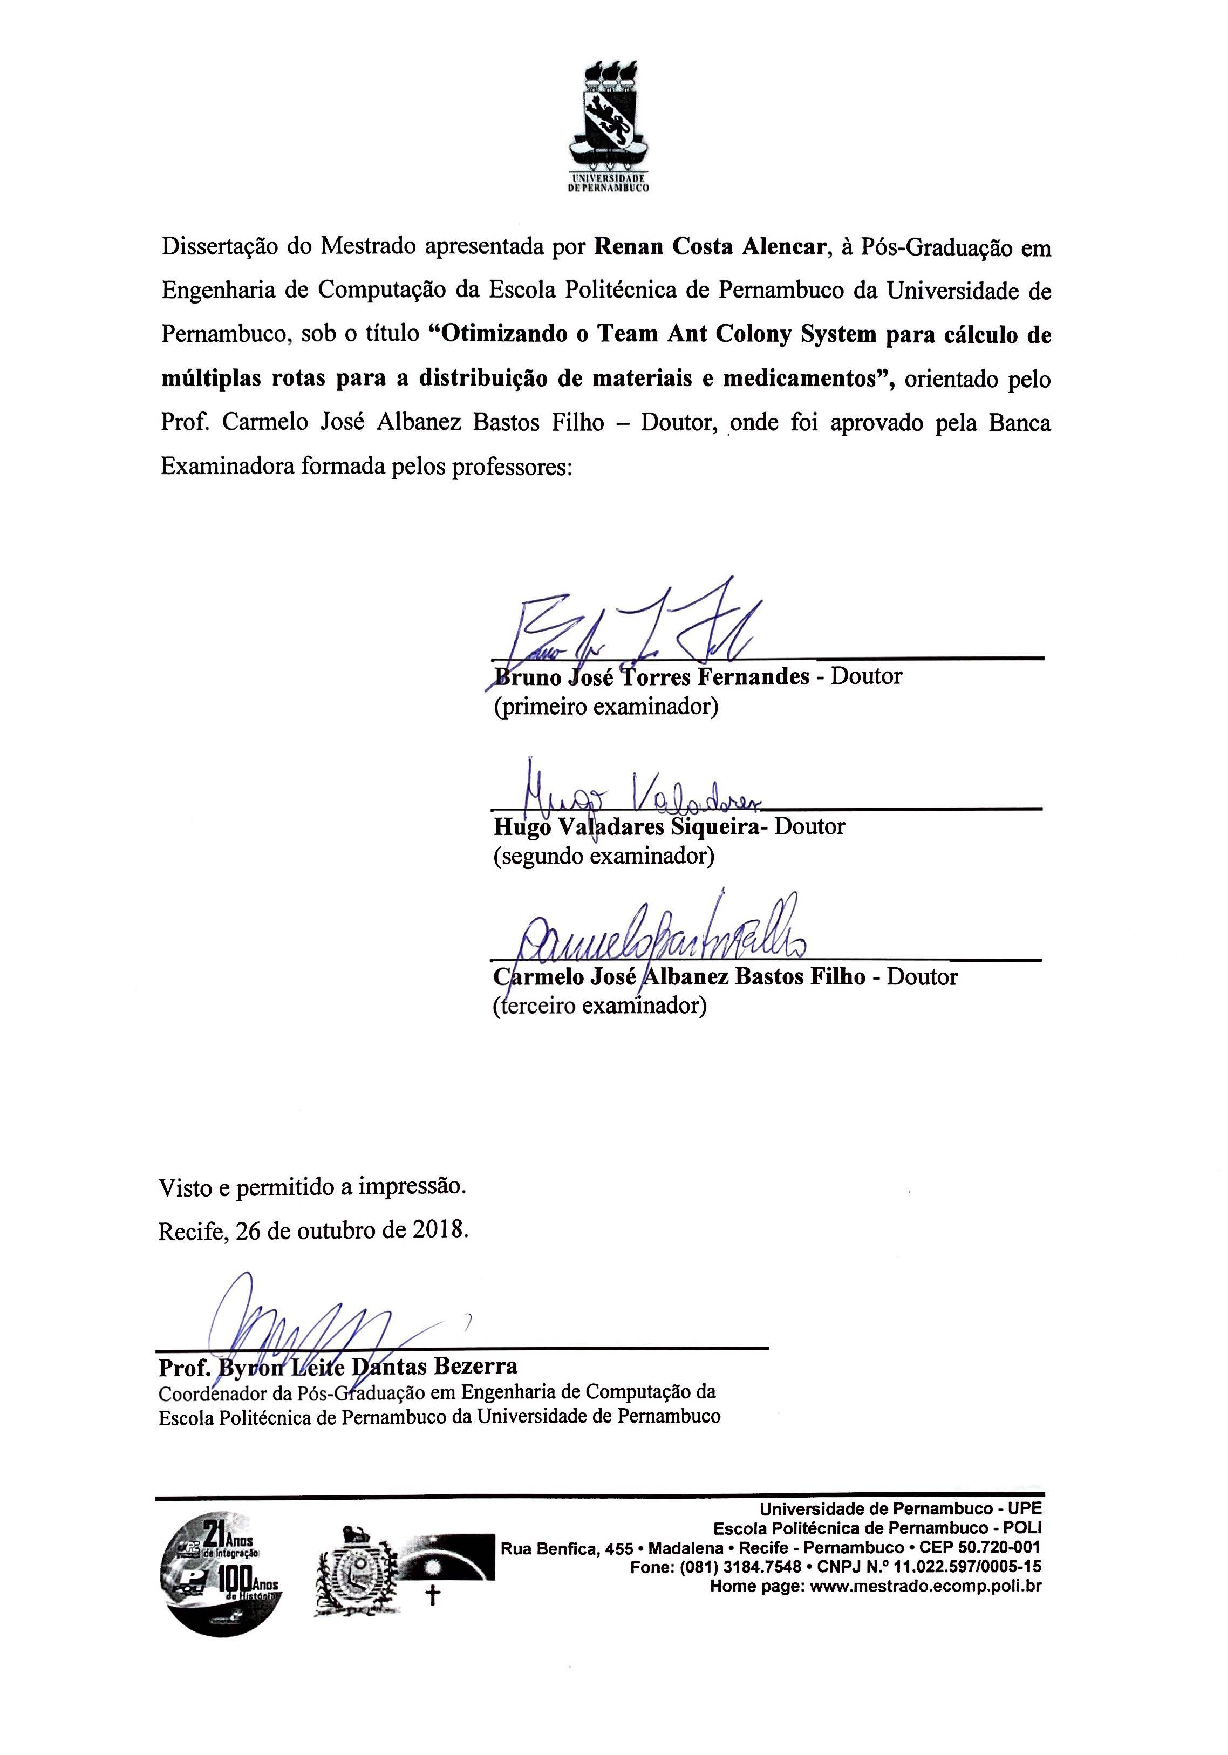
\includepdf{folhadeaprovacao_final.pdf}
%

% ---

% ---
% Dedicatória
% ---

\begin{dedicatoria}
   \vspace*{\fill}
   \centering
   \noindent
   \textit{Dedico este trabalho primeiramente ao Pai Celestial, por ser essencial em minha vida, meu guia, socorro presente na horas de angústia, aos meus pais, aos meus irmãos, aos amigos que fiz nesta jornada e ao meu amor. } \vspace*{\fill}
\end{dedicatoria}

% ---

% ---
% Epígrafe
% ---
\begin{epigrafe}
    \vspace*{\fill}
	\begin{flushright}
“Deus nos concede, a cada dia, uma página de vida nova no livro do tempo. \\Aquilo que colocarmos nela, corre por nossa conta.” \\Chico Xavier
	\end{flushright}
\end{epigrafe}
% ---

% ---
% RESUMOS
% ---

% resumo em português
\setlength{\absparsep}{18pt} % ajusta o espaçamento dos parágrafos do resumo
\begin{resumo}
  A distribuição de remédios e suprimentos hospitalares é considerado um problema complexo e difícil de resolver. Dentro da logística hospitalar, esse problema está associado ao MTSP (\textit{Multiple Traveling Salesman Problem}) e ao KP (\textit{Knapsack Problem}). Os problemas do MTSP visam minimizar o deslocamento total dos caixeiros, com uma restrição de que os caminhos devem começar e terminar no depósito e todos os nós intermediários devem ser visitados uma única vez. Por outro lado, as instâncias do KP visam maximizar a capacidade de uma mochila através de objetos previamente selecionados. Esses problemas podem ser resolvidos usando o \textit{Team Ant Colony Optimization} (TACO), uma variação do algoritmo \textit{Ant Colony System} (ACS), baseado no comportamento das colônias de formigas. O TACO possui \textit{N} equipes com \textit{m} elementos, em que cada formiga de uma equipe corresponde a um vendedor na construção de uma solução para os problemas de MTSP ou KP. No que toca aos resultados, a abordagem acima foi promissora para dois cenários: minimizar a maior rota, alocar uniformemente a carga de trabalho a todos os caixeiros e minimizar o custo total das rotas, ou seja, a soma de todos os custos de rota de caixeiros individuais. No entanto, esses objetivos são concorrentes. O presente trabalho propõe o uso de algoritmos de otimização de enxames como otimizadores globais para obter melhores resultados do que os achados anteriormente. O algoritmo TACO usa esses algoritmos como otimizadores globais para ajustar os seus parâmetros e, consequentemente, melhorar os resultados para os objetivos já mencionados. Os resultados para o uso de otimizadores globais foram promissores para a otimização dos objetivos abordados pela TACO.

  \textit{Palavras-Chave: Problema de Múltiplos Caixeiros Viajantes, Problema da Mochila, Inteligência de Enxames e Logística Hospitalar.}

\end{resumo}

% resumo em inglês
\begin{resumo}[Abstract]
 \begin{otherlanguage*}{english}
  Distributing medicine and hospital supplies is considered a complex and hard problem to solve. Within hospital logistics, that problem is associated with the Multiple Traveling Salesman Problem (MTSP) and the Knapsack Problem (KP). MTSP problems aim to minimize the total displacement of the salesmen, with a constraint that the paths must begin and end in the depot and all intermediate nodes should be visited once. In the order hand, KP instances aim to maximize the capacity of a sack through previously selected objects. Those problems can be solved using the Team Ant Colony Optimization (TACO), a variation of the Ant Colony System (ACS) algorithm, based on ant colony behavior. TACO has N ant teams with m elements, where each ant of a team corresponds to a salesman in the construction of a solution to the MTSP or KP problems. In the results, the above approach was promising for two scenarios: minimizing the largest route, uniformly allocating the workload to all salesmen, and minimizing the total cost of routes, i.e., the sum of all route costs of individual salesmen. However, these objectives are concurrent. This work proposes the use of swarm optimization algorithms as global optimizers to obtain better results than those previous findings. TACO algorithm uses those algorithms as global optimizers to adjust its parameters and consequently to improve the results for those objectives already mentioned. The results for the use of global optimizers were promising for the optimization of the objectives tackled by TACO.

  \textit{Keywords: Multiple Salesmen Travelling Problem, Knapsack Problem, Swarm Intelligence and Hopistal Logistics.}

   \vspace{\onelineskip}
 
   \noindent 
 \end{otherlanguage*}
\end{resumo}

% resumo em francês 
% \begin{resumo}[Résumé]
%  \begin{otherlanguage*}{french}
%     Il s'agit d'un résumé en français.
 
%  \end{otherlanguage*}
% \end{resumo}

% resumo em espanhol
% \begin{resumo}[Resumen]
%  \begin{otherlanguage*}{spanish}
%    Este es el resumen en español.
  
%  \end{otherlanguage*}
% \end{resumo}
% ---



% ---
% inserir o sumario
% ---
\pdfbookmark[0]{\contentsname}{toc}
\tableofcontents*
\cleardoublepage
% ---


% ---
% inserir lista de ilustrações
% ---
\pdfbookmark[0]{\listfigurename}{lof}
\listoffigures
\cleardoublepage
% ---

% ---
% inserir lista de tabelas
% ---
\pdfbookmark[0]{\listtablename}{lot}
\listoftables
\cleardoublepage
% ---

% ---
% inserir lista de siglas e simbolos
% ---

\begin{simbolos}
    \addcontentsline{toc}{chapter}{\listadesimbolosname}
    \item[$ \Gamma $] Letra grega Gama
    \item[$ \Lambda $] Lambda
    \item[$ \zeta $] Letra grega minúscula zeta
    \item[$ \in $] Pertence
\end{simbolos}
\begin{siglas}
	\addcontentsline{toc}{chapter}{\listadesiglasname}
	
  % \item[ABNT] Associação Brasileira de Normas Técnicas
  % \item[abnTeX] ABsurdas Normas para TeX
  % \item[$ \Gamma $] Letra grega Gama
  % \item[$ \Lambda $] Lambda
  % \item[$ \zeta $] Letra grega minúscula zeta
  % \item[$ \in $] Pertence

  \item[AFSA] Artificial Fish-Swarm Algorithm
  \item[ACO] Ant Colony Optimization
  \item[ACS] Ant Colony System 
  \item[CAF] Centro de Abastecimento Farmacêutico
  \item[CEC] Conference on Commerce and Enterprise Computing 
  \item[CTR] Custo Total das Rotas
  \item[DP] Desvio Padrão 
  \item[EA] Arquivo Externo
  \item[FSS] Fish School Search
  \item[GA] Genetic Algorithm
  \item[GRASP] Greedy Randomized Adaptive Search Procedures
  \item[IE] Inteligência de Enxames
  \item[KP] Knapsack Problem
  \item[MGA] Modified Genetic Algorithm
  \item[MOEA/D] Multiobjective Evolutionary Algorithm Based on Decomposition
  \item[MOFSS] Multi-Objective Fish School Search
  \item[MTSP] Multiple Travelling Salesmen Problem
  \item[OG] Otimizador Global
  \item[PRV] Problema de Roteamentode Veículos
  \item[PSO] Particle Swarm Optimization
  \item[RAF] Regra de Atualização do Feromônio
  \item[RTE] Regra de Transaçãode Estado
  \item[RML] Rota Mais Longa
  \item[SMPSO] Speed-constrained Multi-objective PSO
  \item[SPEA2] Strength Pareto Evolutionary Algorithm 
  \item[STACS] Single Team Ant Colony System
  \item[STRBAS] Single Team Rank-Based Ant System 
  \item[SUS] Sistema Único de Saúde 
  \item[TACO] Team Ant Colony Optimization
  \item[TSP] Travelling Salesman Problem
  \item[TSPLIB] Travelling Salesman Problem Library
  \item[UKP] Unbounded Knapsack Problem
                        
\end{siglas}

% ---



% ---
% Agradecimentos
% ---
\begin{agradecimentos}

Primeiramente ao Pai Celestial que permitiu que tudo isso acontecesse, ao longo de minha vida, e não somente nestes anos como mestrando, mas que em todos os momentos é o maior mestre que alguém pode conhecer.

Meus estimados agradecimentos:

À UPE pelo ambiente criativo e amigável que proporciona.

Ao meu orientador prof. Carmelo José Albanez Bastos Filho, pelo empenho dedicado à elaboração deste trabalho, pelas palavras amigas, pela força e motivação que me fizeram enxergar a luz no fim do túnel e, principalmente, a paciência dispendida durante o processo.

Agradeço a minha mãe, heroína que me dá apoio, incentivo nas horas difícies, de desânimo e cansaço.

Ao meu pai, por quem tomo como exemplo de vida, quem me ensinou a sempre fazer o correto e por ter me dado a melhor herança da vida terrena: o conhecimento.

Obrigado aos meus irmãos, que nos momentos de minha ausência dedicados à vida acadêmica e ao trabal, sempre fizeram entender que o futuro é feito a partir da constante dedicação no presente.

Aos amigos que fiz durante esta jornada e aos amigos que sempre me acompanham nas minhas jornadas de vida.

Ao meu amor que é a minha base mais sólida, que sempre me motiva e que sempre divido os bons e os momentos difíceis.

\end{agradecimentos}
% ---


% ----------------------------------------------------------
% ELEMENTOS TEXTUAIS
% ----------------------------------------------------------
\textual
\pagestyle{simple}
\aliaspagestyle{chapter}{simple}


\chapter{Introdução}
% ----------------------------------------------------------

% Este documento e seu código-fonte são exemplos de referência de uso da classe
% \textsf{abntex2} e do pacote \textsf{abntex2cite}. O documento
% exemplifica a elaboração de trabalho acadêmico (tese, dissertação e outros do
% gênero) produzido conforme a ABNT NBR 14724:2011 \emph{Informação e documentação
% - Trabalhos acadêmicos - Apresentação} \cite{NBR14724:2011}.
% A expressão ``Modelo Canônico'' é utilizada para indicar que \abnTeX\ não é
% modelo específico de nenhuma universidade ou instituição, mas que implementa tão
% somente os requisitos das normas da ABNT. Uma lista completa das normas
% observadas pelo \abnTeX\ é apresentada em \cite{abntex2classe}.

% Sinta-se convidado a participar do projeto \abnTeX! Acesse o site do projeto em
% \url{http://www.abntex.net.br/}. Também fique livre para conhecer,
% estudar, alterar e redistribuir o trabalho do \abnTeX, desde que os arquivos
% modificados tenham seus nomes alterados e que os créditos sejam dados aos
% autores originais, nos termos da ``The \LaTeX\ Project Public
% License''\footnote{\url{http://www.latex-project.org/lppl.txt}}.

% Encorajamos que sejam realizadas customizações específicas deste exemplo para
% universidades e outras instituições --- como capas, folha de aprovação, etc.
% Porém, recomendamos que ao invés de se alterar diretamente os arquivos do
% \abnTeX, distribua-se arquivos com as respectivas customizações.
% Isso permite que futuras versões do \abnTeX~não se tornem automaticamente
% incompatíveis com as customizações promovidas. Consulte
% \cite{abntex2-wiki-como-customizar} par mais informações.

% Este documento deve ser utilizado como complemento dos manuais do \abnTeX\
% \cite{abntex2classe,abntex2cite,abntex2cite-alf} e da classe \textsf{memoir}
% \cite{memoir}.

% Esperamos, sinceramente, que o \abnTeX\ aprimore a qualidade do trabalho que
% você produzirá, de modo que o principal esforço seja concentrado no principal:
% na contribuição científica.

% Equipe \abnTeX

% Lauro César Araujo

O Problema do Caixeiro Viajante (\textit{Travelling Salesman Problem} - TSP) e o Problema da Mochila (\textit{Knapsack Problem} - KP) são dois dos problemas de otimização combinatória mais estudados nas últimas quatro décadas, de acordo com Augustine (2002) \cite{augustine2002offline} Bektas (2006) \cite{bektas2006multiple}, Lin (2007) \cite{lin2008solving} e Vallivaara \cite{vallivaara2008team}. Estes autores afirmam que tais problemas se destacam de outros problemas combinatórios por serem fáceis de projetar, mas difíceis de resolver. Assim, o TSP e o KP pertencem ao conjunto de problemas NP-completos. Embora sejam difíceis de resolver, mesmo separadamente, existem alguns problemas reais que podem ser mapeados como uma combinação TSP-KP, resultando em uma tarefa complexa.

De acordo Bektas (2006) \cite{bektas2006multiple}, há uma infinidade de problemas da vida real que podem ser encarados como problemas MTSP (\textit{Multiple Trvaelling Salesmen Problem}, uma variação multi-objetiva do problema clássico TSP), e.g., na resolução de PRVs (Problema de Roteamento de Veículos) com adição de restrições às soluções. Na definição básica do MTSP, há $m > 1$ caixeiros inicialmente posicionados numa mesma cidade, definida como depósito. As demais cidades da instância são denominadas de intermediárias. O MTSP tem por objetivo minimizar o deslocamento total dos caixeiros, com a restrição de que os caminhos devem começar e terminar no depósito e todas as cidades intermediárias devem ser visitadas uma única vez. No caminho de cada caixeiro deve existir ao menos uma cidade além do depósito.

O KP é um problema combinatório, que aloca espaço em uma mochila, com antecedência, de acordo com uma seleção de objetos. Assim, o valor total de todos os objetos escolhidos é maximizado na mochila. Lin (2007) \cite{lin2008solving} afirma que o KP é um problema muito frequente e que aparece no mundo real em diversos seguimentos, e.g., no planejamento econômico e na indústria, como problemas de carga, corte de estoque e empacotamento de lixo. Martello e Toth (1990) \cite{Martello:1990:KPA:98124} definem o problema do KP como um vetor $n$-objeto de variáveis binárias $x_i$ ($i = 1,…, n$), no qual o objeto $i$ tem um peso $w_i$ e a mochila tem uma capacidade $M$. Se uma fração $x_i$; $0 \leq xi \leq 1$ é colocado na mochila, então um lucro, $g_i x_i$, é o ganho. O KP visa encontrar uma combinação de objetos que maximize o lucro total de todos os objetos escolhidos na mochila. Enquanto a capacidade da mochila é $M$, o peso total de todos os objetos escolhidos deve ser no máximo $M$.

Embora ter esses dois problemas associados não seja incomum, eles podem aparecer em cenários complexos. Por exemplo, a distribuição de medicamentos em grandes centros hospitalares pode ser vista como uma instância do MTSP-KP. Tanto a separação (KP) quanto a distribuição (MTSP) têm um alto número de combinações e, mesmo separadas, essas tarefas são difíceis de serem otimizadas, exigindo ferramentas sofisticadas para lidar com elas. Como garantidor da segurança do paciente, Ribeiro (2005) \cite{ribeiro_2005} explica que a logística hospitalar é um dos maiores desafios encontrados pelos gestores dos hospitais, principalmente no que diz respeito ao atendimento das necessidades organizacionais de forma rápida, correta e eficiente. Além disso, Souza et al. (2013) \cite{de2013logistica} explica que, para um hospital público no Brasil, em que o orçamento se restringe aos recursos financeiros disponibilizados pelo Sistema Único de Saúde (SUS), é fundamental que esses recursos sejam implantados com eficiência.

Algumas abordagens, baseadas em métodos matemáticos, algoritmos evolutivos e inteligência de enxames, são usadas para otimizar instâncias de MTSP e KP. É possível citar os seguintes exemplos: Algoritmo Genético - GA (HOLLAND, 1992) \cite{holland1992genetic}, \textit{Ant Colony Optimization} - ACO (DORIGO et al., 2008) \cite{dorigo2008particle} e \textit{Artificial Bee Colony} - ABC (KARABOGA, 2005) \cite{karaboga2005idea}. Essas abordagens visam resolver problemas de produção de aço (TANG et al., 2000) \cite{tang2000multiple}, distribuição de cigarros (LIU et al., 2009) \cite{liu2009ant}, ordens de serviço (BARBOSA; KASHIWABARA, 2015, 2016) \cite{barbosa2015aplicaccao, barbosa2016aplicaccao}, roteamento de redes de sensores (WANG et al., 2007) \cite{wang2007hierarchical}, entre outros.

Durante a revisão sistemática sobre o tema, não foram encontrados estudos relacionados ao uso de processos de otimização global para melhorar o desempenho de meta-heurísticas implementadas para resolver o problema MTSP-KP. Assim, ainda há espaço para otimizar os parâmetros do MTSP-KP com algoritmos meta-heurísticos visando atingir objetivos específicos, especialmente quando é necessário balancear o tamanho das rotas e o número de entregas por caixeiro simultaneamente. Logo, este trabalho propõe uma metodologia para otimizar os parâmetros do MTSP através de otimizadores baseados em população global, e.g., algoritmos baseados em inteligência de enxames. Utilizamos como estudo de caso um processo de distribuição de medicamentos com múltiplas rotas.

% ---
\section{Motivação}
\label{sec-motivacao}
% ---

Uma forma de resolver problemas combinatórios é simplesmente enumerar todas as soluções possíveis e guardar aquela de menor custo. Entretanto, essa é uma ideia ingênua pois para qualquer problema NP-difícil, i.e., um problema útil e real, esse método torna-se impraticável, já que o conjunto de soluções possíveis é inviável de ser calculado. Mesmo que seja utilizado um supercomputador para resolver o problema, o tempo de processamento pode levar várias horas, ou vários dias ou até anos. Como consequência, os problemas práticos dessa natureza fazem parte do cotidiano da sociedade moderna. Os problemas aqui tratados são conhecidos tecnicamente por NP-difícil. Portanto, técnicas computacionais mais apuradas são necessárias para resolver os problemas desta classe.

Há uma infinidade de tarefas da vida real que podem ser encarados como problemas de Otimização Combinatória. A Otimização Combinatória tem uma gama de aplicações possíveis como na resolução de problemas de Roteirização de Veículos, Ensalamento em Escolas e Universidades (\textit{Timetabling}), Escalonamento de Trabalho Humano, Escalonamento de Tarefas em Máquinas, Projeto de Circuitos Integrados, Projeto de Redes com Restrições de Conectividade, dentro outros citados por Papadimitriou e Steiglitz (1998) \cite{papadimitriou1982combinatorial}. Todavia, problemas do mundo real tendem a envolver vários objetivos que precisam ser resolvidos ao mesmo tempo, e que, em geral, são conflitantes entre si. Nestes casos, de acordo Branke et al. (2008) \cite{branke2008multiobjective}, não será encontrada apenas uma única solução, mas sim varias soluções possíveis, que representarão uma curva, chamada de Soluções de Pareto, definida por Collette e Siarry (2013) \cite{collette2013multiobjective}. Esta definição é detalhada no capítulo seguinte. 

A resolução de um problema de otimização normalmente passa por duas fases. A primeira fase consiste em transformar o problema em um modelo. Posteriormente, na segunda fase, um algoritmo deve ser implementado para resolvê-lo. Nem sempre é possível encontrar a melhor solução de um problema de otimização em tempo razoável por meio de algoritmos exatos. Nesses casos, um bom candidato pode ser suficiente para a aplicação que se tem em mãos. De acordo com Murakami 2008 \cite{murakami2008soluccao}, os Métodos Heurísticos são algoritmos que não garantem encontrar a solução ótima de um problema, mas são capazes de retornar uma solução de qualidade em um tempo adequado para as necessidades da aplicação.

Meta-heurísticas são paradigmas de desenvolvimento de algoritmos heurísticos. Diversas propostas surgiram nos últimos anos impulsionadas pelos problemas pertencentes à classe NP-difícil. Dentre as mais conhecidas podemos destacar Algoritmos Genéticos (GA, \textit{Genetic Algorithms}), inspirados na evolução natural dos seres vivos; Otimização por Colônia de Formigas (ACO, \textit{Ant Colony Optimization}), algoritmos baseados no comportamento das formigas para encontrar comida; \textit{Simulated Annealing}, baseada originalmente em conceitos de Mecânica Estatística considerando a analogia entre o processo físico annealing de sólidos e a resolução de problemas de otimização combinatória; Busca Tabu, utiliza mecanismos de memória e diversificação das soluções como recursos para encontrar a solução ótima; e GRASP (\textit{Greedy Randomized Adaptive Search Procedures}), técnica baseada no paradigma da busca gulosa (ou míope).

O algoritmo FSS (\textit{Fish School Search}), criado por Bastos-Filho \cite{bastos2008novel}, foi introduzido em 2008 com o objetivo de abordar tarefas de otimização em espaços de busca multimodais. A principal vantagem deste algoritmo é a capacidade de autorregulação, o trade-off entre exploração e explotação. Alguns resultados preliminares, publicados por Bastos-Filho (2009) \cite{bastos2009fish}, indicam que o FSS pode superar alguns dos algoritmos baseados em enxames em funções de benchmark com espaços de busca multimodais. Entretanto, não há variante do algoritmo que trate da resolução de problemas combinatórias.

% ---
\section{Objetivos}
\label{sec-objetivos}
% ---

O problema de logística na distribuição de medicamentos em hospitais de grande porte apresenta múltiplos demandantes (farmácias menores) bem como múltiplos despachantes (entregadores), tendo um único depósito chamado de CAF – Centro de Abastecimento Farmacêutico. Logo, pode ser abordado de três modos distintos: agrupando os demandantes e em seguida encontrando os caminhos para distribuição; encontrando os caminhos de distribuição primeiro e depois distribuindo os demandantes; ou realizando um processo de agrupamento e roteamento em conjunto. Para este trabalho será utilizado a primeira abordagem devido a sua facilidade na resolução da tarefa foco deste trabalho haja vista que a segunda abordagem faz a associação entre a resolução de problemas MKP (Problema de Múltiplas Mochilas) com instâncias MTSP que será tratado em trabalhos futuros.

Neste trabalho é proposto o uso de uma metodologia para resolução de problemas de MTSP, que visa a distribuição de medicamentos, otimizando a programação de percursos para a entrega. A partir de um cenário hospitalar, são construídas instâncias de MTSP. As posições das entregas a serem executadas representam as cidades da instância e os entregadores de pedidos representam os caixeiros.

Estas instâncias são otimizadas pela abordagem TACO – \textit{Team Ant Colony Optimization}, algoritmo proposto por Vallivaara (2008) \cite{vallivaara2008team}, para distribuição de medicamentos a material hospitalar bem como os percursos a serem realizados pelos entregadores. As melhores soluções geradas pela TACO são utilizadas para definir a distribuição das ordens entre os entregadores e os percursos que devem ser realizados.

Ao fim do processo de encontro das soluções, um otimizador global é utilizado, baseado em algoritmos de base populacional como os algoritmos de enxames. Esta associação visa otimizar soluções previamente encontradas em relação minimização do custo no deslocamento dos entregadores (minimização do tempo de entrega) bem como o balanceamento de atendimentos realizados por eles (maximização do número de atendimento).

A abordagem TACO foi escolhida devido aos resultados encorajadores para o MTSP e vem sendo aplicado com sucesso para vários problemas NP-difíceis (problemas não polinomiais) de otimização combinatória; e a fim de explorar novas formas de aplicá-la ao MTSP. Também os algoritmos de enxames foram escolhidos devido as suas características de grande poder de otimização dos parâmetros inerentes ao TACO.

A partir do problema exposto na seção anterior e da proposta acima descrita, esta pesquisa tem como objetivo fomentar os estudos escassos na resolução de problemas de logística voltados a área hospitalar e que possa contribuir para a melhoria da gestão. É objetivo também desta pesquisa contribuir com a resolução de problemas combinatórios como o MTSP e o campo dos métodos computacionais, como a Inteligência de Enxames.

% ---
\section{Estrutura da Dissertação}
\label{sec-estrutura}
% ---

Esta dissertação está estruturada em 7 capítulos, iniciando neste Capítulo 1 com uma introdução sobre a proposta apresentada. No Capítulo 2, é introduzido uma descrição básica dos problemas TSP e KP e suas variantes. No Capítulo 3, é descrito alguns algoritmos baseados em inteligência de enxame para resolver problemas combinatórios. No Capítulo 4, é apresentado os trabalhos relacionados envolvendo algoritmos meta-heurísticos para resolver instâncias de MTSP e KP. No Capítulo 5, são explanados o modelo proposto, a instância do problema a ser otimizada e os cenários e suas configurações para minimizar a instância. No Capítulo 6, é apresentada uma discussão dos resultados otimizados fazendo uma comparação entre os otimizadores globais baseados em população. Finalmente, no Capítulo 7, o último deste trabalho, é destacado algumas conclusões sobre o modelo proposto e trabalhos futuros.
\chapter{Problemas Combinatórios}

% \lipsum[1-2]

% FALTA AJUSTAR \subsubsubsection{Exemplo subsubsubsection}

Lacerda (2012) \cite{de2012nova} define que os problemas de Otimização Combinatória, em geral, se resumem a encontrar, dentre todos os possíveis subconjuntos de soluções, aquela cujo o custo seja o menor possível. Isto é, suponha que há um conjunto de itens e uma série de regras que podem ser usadas para selecionar alguns elementos (itens desse conjunto). Usando essas regras, há várias maneiras diferentes de escolher os elementos e criar outros conjuntos menores (subconjuntos). Se cada elemento estiver associado à um custo, os subconjuntos criados também terão um custo que é dado, por exemplo, pela soma dos custos de seus elementos.

Uma forma de resolver tais tarefas seria simplesmente enumerar todas as soluções possíveis e guardar aquela de menor custo, segundo Bektas (2006) \cite{bektas2006multiple}. Entretanto, essa é uma ideia ingênua pois para qualquer problema de um tamanho interessante (e útil), esse método torna-se impraticável, já que o número de soluções possíveis é muito grande. Mesmo que, para a sua resolução, se utilize um supercomputador, haveria um custo computacional muito elevado.

Segundo Martello e Toth (1990) \cite{Martello:1990:KPA:98124}, modelos baseados em grafos são imensamente utilizados em muitos exemplos de otimização combinatória. Grafo é uma forma de representar um conjunto de elementos e suas relações. Esse recurso é muito utilizado para modelagem de instâncias por ser uma forma bastante intuitiva para representá-las. Além disso, na literatura podem ser encontrados algoritmos para resolver diversos otimizações combinatórias em grafos. Um exemplo de problema modelado em forma de grafo é o do Caixeiro Viajante (do inglês, \textit{Travelling Salesman Problem}). O caixeiro visa encontrar a menor rota entre cidades onde obedeçam às restrições de ser o menor caminho e que ele venha passar no máximo uma única vez em cada cidade do seu trajeto.

Segundo Papadimitriou e Steiglitz (1998) \cite{papadimitriou1982combinatorial}, otimização combinatória é a ciência de encontrar a melhor solução de um conjunto grande, mas finito de soluções possíveis. Este grande número de possibilidades vem da necessidade de encontrar um bom subconjunto de elementos de um dado conjunto sujeito a algumas regras. O custo ou qualidade de uma solução é geralmente definido como uma função desses elementos.

Enquanto na maioria das aplicações práticas de exploração através de todos os casos é apenas uma possibilidade teórica, devido ao seu número imenso, a otimização combinatória tenta oferecer métodos e algoritmos mais sofisticados, resultando em tempos de execução razoável. Algumas das ferramentas mais poderosas para encontrar soluções ótimas são programação linear e integral e programação de restrição.

Para aqueles casos em que essas técnicas não conseguem encontrar boas soluções em tempo razoável, algumas outras abordagens são possíveis, como algoritmos de Aproximação, heurística e métodos de limites duplos, como aponta Malaquias (2006) \cite{malaquias2006uso}.

% ---
\section{O Problema do Caixeiro Viajante (TSP)}
\label{sec-tsp}
% ---

De acordo com Bektas (2006) \cite{bektas2006multiple} e Silva (2016) \cite{silva2016algoritmo}, o Problema do Caixeiro Viajante (TSP) é considerado um dos exemplos de otimização combinatória mais estudado por pertencer à classe dos problemas NP-completos. O TSP é de fácil descrição, mas de difícil resolução devido a sua explosão combinatória, ou seja, há zilhões de possibilidades de se resolvê-lo. Tem como desafio encontrar o caminho mais curto visitando cada membro de uma coleção de locais e retornando ao seu ponto de partida (Figura \ref{fig:tsp-sample}). Logo, o torna intratável na obtenção de soluções exatas. Bektas afirma que o problema tem uma aplicabilidade em diversas áreas tais como: indústrias (minimizar custo por meio da melhor rota utilizada por equipamentos no processo de montagem), empresas (transportadoras, entrega e coleta de cargas), automobilística (redução de custo de viagem), transporte de passageiros, roteirização de serviços de reparos ou serviços públicos (como coleta de lixo, entrega postal), sequenciamento de genoma.

\begin{figure}[h]
	\caption{\label{fig:tsp-sample}Problema do caixeiro-viajante}
	\begin{center}
	    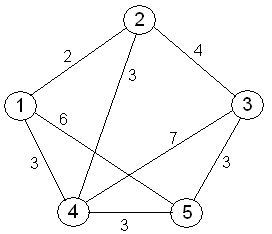
\includegraphics[scale=0.5]{imagens/tsp-sample.jpg}
	\end{center}
	\legend{Fonte: Google Images}
\end{figure}


O TSP pode ser representado por um grafo completo $G = (N, A)$, com $N$ sendo o conjunto de nós, também chamado cidades, e $A$ sendo o conjunto de arcos totalmente conectados aos nós. Cada arco $(i, j)$ pertencente $A$ é atribuído um valor $d_ij$ que representa a distância entre as cidades $i$ e $j$.

Tomando o exemplo da Figura \ref{fig:tsp-sample}, temos um grafo de cinco vértices em que cada aresta, associada a um vértice, possui um peso. Pensando em encontrar o percurso que passe em todos nós uma única vez, temos duas possíveis soluções ilustradas na Figura \ref{fig:tsp-exemplo}. É possível perceber que, ao somar o peso de todas as arestas do percurso, a rota ilustrada a esquerda possui menor tamanho se comparado a da direita. 

\begin{figure}[h]
	\caption{\label{fig:tsp-exemplo}Visualização de soluções em grafo.}
	\begin{center}
	    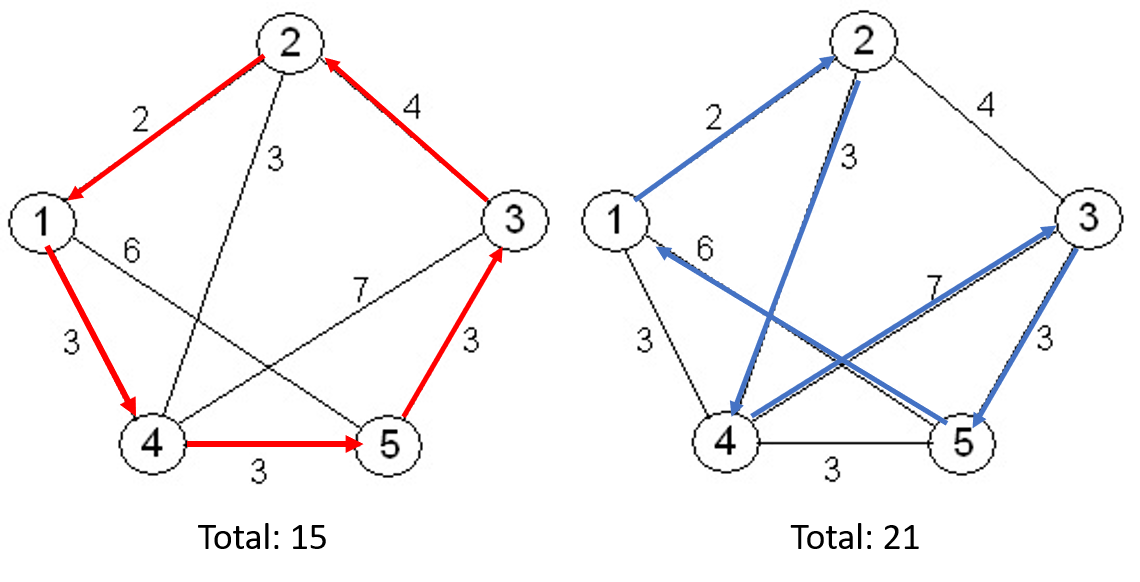
\includegraphics[scale=0.5]{imagens/grafos.png}
	\end{center}
	\legend{Fonte: O próprio autor}
\end{figure}

Logo, o TSP é um problema de encontrar um caminho fechado mais curto visitando cada um dos $n = |N|$ nós de $G$ exatamente uma vez. Para insâncias de TSP simétricos, as distâncias entre as cidades são independentes da direção transversal dos arcos, isto é, $D_ij = d_ji$ para cada par de nós. No TSP assimétrico pelo menos para um par de nós temos $d_ij \leq d_ji$.

% ---
\section{O Problema da Mochila (KP)}
\label{sec-kp}
% ---

O problema da mochila (KP) pode ser enunciado da seguinte forma (MARTELLO; TOTH, 1990) \cite{Martello:1990:KPA:98124}:

\textit{Um viajante levará consigo apenas uma mochila para sua viagem (Figura \ref{fig:kp-sample}). Sua mochila possui uma dada capacidade e deve ser preenchida com alguns objetos que lhe sejam úteis durante a viagem. Cada objeto possui um peso e um dado valor para o viajante e este possui apenas uma unidade de cada objeto a ser escolhido. Quais objetos devem ser levados pelo viajante em sua mochila de forma a maximizar o valor da mochila?}

\begin{figure}[h]
	\caption{\label{fig:kp-sample}Problema da mochila: Como maximizar o valor com um peso máximo?}
	\begin{center}
	    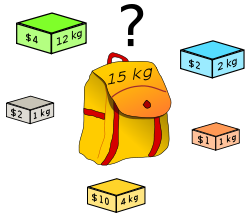
\includegraphics[scale=0.5]{imagens/kp-sample.png}
	\end{center}
	\legend{Fonte: Google Images}
\end{figure}

Seja $w_j$ o peso do $j$-ésimo objeto e $p_j$ seu valor. Se o objeto $x_j$ aparece na mochila, então  $x_j=1$ caso contrario $x_j=0$. Se denotarmos por $c$ a capacidade da mochila, e por $n$ a quantidade de objetos disponíveis para escolha e $F_(c)$ como o maior valor obtido para a mochila de capacidade $c$ usando os $n$ objetos, então o problema pode ser formulado algebricamente como a seguir:

\begin{equation} \label{eq:taco-ret} 
F_{(c)} = max\sum_{j=1}^{n} p_{j}x_{j} \quad (p_{j} > 0 )
\end{equation}

\begin{equation} \label{eq:taco-ret} 
sujeito \quad a\sum_{j=1}^{n} w_{j}x_{j} \leq c \quad (w_{j},c > 0 )
\end{equation}

onde: $x_j=0$ ou $x_{j}=1$.

Esta versão do problema é conhecida como problema da mochila binária (\textit{Binary KP} ou \textit{0-1KP}); Martello e Toth 1990 \cite{Martello:1990:KPA:98124}.

Se permitirmos a \(x_{j}\) assumir qualquer valor inteiro maior que zero então temos a forma mais genérica da versão unidimensional do problema da mochila. De acordo com a definição presente no trabalho de Martello e Toth 1990 \cite{Martello:1990:KPA:98124}, tal problema é conhecido como problema da mochila ilimitada (\textit{Unbounded Knapsack Problem} ou UKP).

Martello e Toth afirmam que, apesar do nome, o problema da mochila não é útil apenas na solução de problemas de empacotamento. Existem também aplicações na área da criptografia, engenharia naval, gerenciamento de projetos e finanças entre outras.

% ---
\section{Otimização e Problemas Multi-Objetivos}
\label{sec-multi}
% ---

É imprescindível o estudo de problemas multi-objetivo visto que a maior parte dos problemas do mundo real tendem a ser classificados desta forma. Augusutine (2002) \cite{augustine2002offline} explica que a complexidade dos problemas reais que surgem nas sociedades tecnológicas modernas é caracterizada pela existência de múltiplas perspectivas de análise, refletindo aspectos econômicos, sociais, políticos, físicos, de engenharia, administrativos, psicológicos, éticos, estéticos, etc.

Bastos-Filhos e Guimarães (2013) \cite{bastos2015multi} resumem o conceito de otimização como sendo “a busca por soluções para determinado problema (ou problemas) que o satisfaçam da melhor maneira possível”. Collette e Siarry (2013) \cite{collette2013multiobjective}, em seu livro “Multiobjective Optimization: Principles and Case Studies”, definem um problema de otimização como sendo a busca de um mínimo ou máximo (o ótimo) de uma função. O autor também descreve um caso específico de otimização chamado problema de otimização restrita. Este tipo ocorre quando problemas de otimização para os quais as variáveis da função a serem otimizadas são restritas para evoluir em uma área precisamente definida do espaço de pesquisa.

\begin{figure}[htb]
	\centering
	\caption{\label{fig:hotel-multi}Dilema de reserva de um quarto de hotel em função de dois objetivos: preço e conforto.} 
	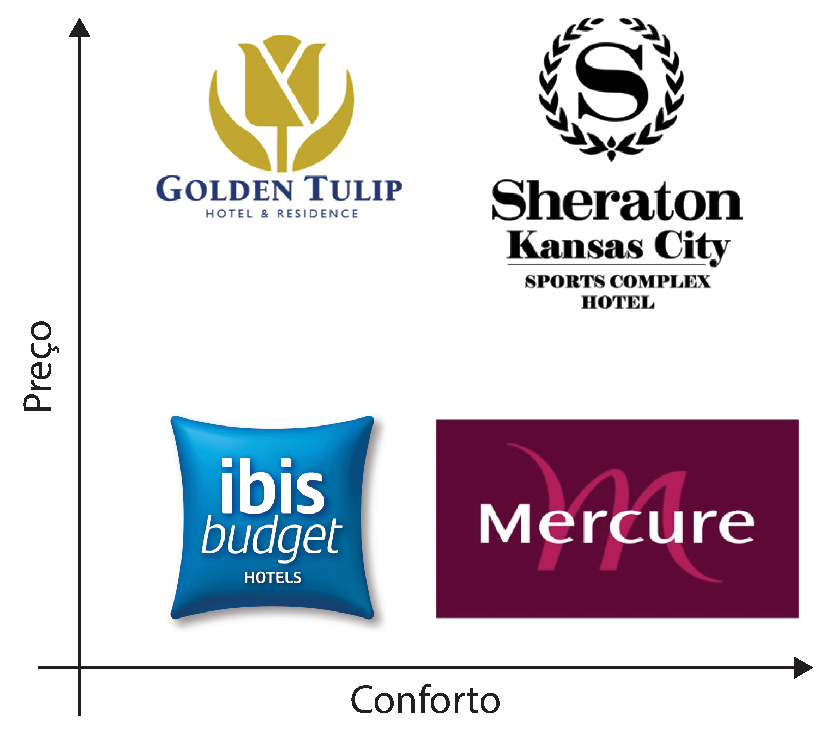
\includegraphics[width=0.5\textwidth]{imagens/hotel-multi.eps}
	\legend{Fonte: o próprio autor.}
\end{figure}

Branke et al. (2008) \cite{branke2008multiobjective} explicam que um problema de otimização mono objetivo envolve uma única função objetivo (ou função \textit{fitness}) e geralmente resulta em uma solução única, chamada de solução ótima. Por outro lado, uma tarefa de otimização multi-objetivo considera vários objetivos conflitantes simultaneamente. Nesse caso, geralmente não há solução ótima única, mas um conjunto de alternativas com diferentes compensações, chamadas de soluções ótimas de Pareto, ou soluções não dominadas.

A Figura \ref{fig:hotel-multi} apresenta um problema para a reserva de hotel, levando em consideração dois objetivos: preço e conforto. Se a pretensão for por um quarto com maior conforto, o preço será mais alto. Já, se pretende um quarto com menor preço, o conforto também será afetado, diminuindo-o.


\chapter{Algorítmos Meta-Heurísticos e Inteligência de Enxames}

As técnicas de Inteligência de Enxames (IE) estão inseridas dentro Computação Evolutiva, apesar de trazer uma metáfora diferente da evolução das espécies. Na IE, o comportamento biológico de seres vivos serve de inspiração o que torna as técnicas de otimização mais simples e fáceis de serem implementadas do que as técnicas evolucionárias.

Chan e Tiwari (2007) \cite{chan2007preface}, em seu livro “Swarm Intelligence: Focus on Ant and Particle Swarm Optimization”, expõem que a complexidade crescente dos problemas exigiu que os pesquisadores encontrassem o possível formas de facilitar a solução dos problemas. Segundo os autores, isso motivou os pesquisadores a compreender ideias da natureza e implantá-lo nas ciências da engenharia. Esse modo de pensar levou a surgimento de muitos algoritmos biologicamente inspirados que provaram ser eficientes em lidar com os problemas computacionalmente complexos com competência, tais como Algoritmo Genético (GA), Otimização de Colônia de Formigas (ACO), Otimização de Enxame de Partículas (PSO), etc.

Na IA, de acordo com Eberhart e Kennedy (2001) \cite{eberhart2001swarm}, o comportamento global do enxame é um efeito emergente das interações locais dos membros do enxame. De acordo com Filho et al. \cite{bastos2008novel}, as informações pessoais e sociais guardam semelhança com operadores de recombinação e de cruzamento, enquanto que a conservação de movimento da partícula atua como uma espécie de mutação direcional. Há diferenças, no entanto, sendo a maior delas o papel da seleção natural: enquanto que métodos evolutivos tem como parte essencial a morte dos indivíduos menos aptos, em um processo social os indivíduos são preservados durante a execução do algoritmo, de forma que o próprio indivíduo se adapta no decorrer do tempo.

Há uma série algoritmos de otimização de problemas que abordam diferentes grupos de seres vivos, desde pássaros a vagalumes para resolver problemas de otimização. Engelbrecht (2006) \cite{engelbrecht2006fundamentals} exemplifica alguns problemas resolvidos pela IE como aproximação de funções, agrupamento, otimização de estruturas mecânicas, resolução de sistemas de equações, otimização de roteamento em redes de telecomunicações, coloração de grafos, programação e resolução do problema de atribuição quadrática, dentro outros. Os problemas aqui tratados são conhecidos tecnicamente por NP-difícil. Portanto, técnicas computacionais mais apuradas são necessárias para resolver esses problemas.


Dentro da IE, há várias técnicas que abordam diferentes grupos de seres vivos desde pássaros a bactérias. Entretanto, este trabalho faz uso das seguintes abordagens: \textit{ Ant Colony Optimization} (ACO), \textit{Particle Swarm Optimization} (PSO) e \textit{Fish School Search} (FSS). O ACO, Otimização por Colônia de Formigas, tem a sociedade organizada das formigas como modelo para busca de alimentos através de rastros deixados pelas formigas. Já o PSO, Otimização por Enxame de Partículas, tem como inspiração os bandos de pássaro, tendo como a forma de voar em grupo na busca de alimento e mecanismo de interação social. Por fim, o FSS, Busca em Cardume de Peixes, tem no movimento do nado dos peixes a inspiração para proteção e busca de locais mais favoráveis para sobrevivência.

% ---
\section{ACO}
\label{sec-aco}
% ---

O ACO, desenvolvido por Dorigo e sua equipe em 1996 \cite{dorigo1996any}, inspirou-se no comportamento de colônias de formigas reais, em particular, por seu comportamento de forrageamento. Uma das principais ideias é a comunicação indireta entre os indivíduos de uma colônia de agentes, chamados de formigas, com base em uma analogia com trilhas de uma substância química, chamada feromônio, que as formigas reais utilizam para a comunicação. As trilhas (artificiais) de feromônio são um tipo de informação numérica distribuída que é modificada pelas formigas para refletir sua experiência acumulada ao resolver um problema particular.

Como descreve Mulati, Constantino e da Silva (2013) \cite{mulati2013otimizaccao}, foi descoberto que a comunicação entre as formigas que caminhavam pela trilha ocorria por meio de uma substância química, denominada feromônio, depositada por elas próprias. Enquanto as formigas caminham por uma trilha, inicialmente de forma aleatória, elas depositam uma certa quantidade de feromônio no solo. Assim, as próximas formigas tomam a decisão de seguir um caminho com probabilidade proporcional à quantidade feromônio depositada anteriormente. Ao decidir seguir um caminho com a presença da substância, ocorre então um reforço do caminho com o seu próprio feromônio. Este comportamento é denominado de auto-catalítico por ser um processo que reforça a si mesmo. O feromônio depositado tende a evaporar com o tempo, então quanto maior é a concentração de formigas passando pelo mesmo lugar, mais atrativo ele se torna para as próximas formigas. A Figura \ref{fig_aco} ilustra um experimento com formigas reais.

\begin{figure}[h]
	\caption{\label{fig_aco}Ilustração do experimento com formigas}
	\begin{center}
	    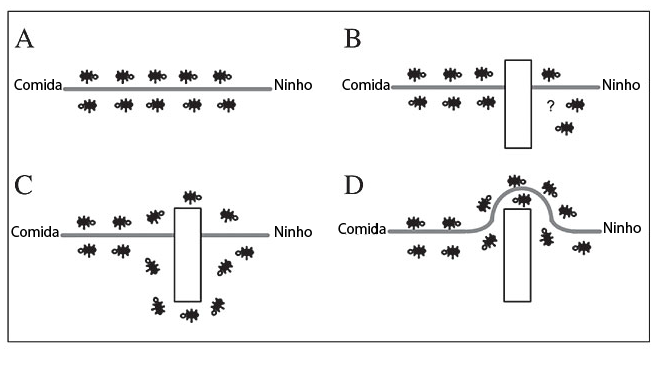
\includegraphics[scale=0.5]{imagens/aco-sample.png}
	\end{center}
	\legend{Fonte: Google Images}
\end{figure}


As formigas conseguem obter um bom caminho entre dois pontos. Na primeira decisão após a inserção do obstáculo, as quantidades de formigas a escolher o caminho mais curto e o caminho mais longo devem ser aproximadamente a mesma, de modo que elas escolhem o caminho com base no feromônio encontrado, sendo que as probabilidades de ambos os lados devem ter valores próximos um do outro. Porém, na segunda decisão, as formigas que percorreram o caminho mais curto já estão voltando, depositando ainda mais feromônio, enquanto as que foram pelo caminho mais longo ainda estão completando a primeira transição. Desta forma, as formigas tendem a seguir caminho mais curto.

De forma análoga, um indivíduo da colônia artificial constrói soluções candidatas, começando com uma solução vazia e, em seguida, adicionando componentes solução de forma iterativa até uma solução candidata completa ser gerada. Após a construção da solução estar completa, as formigas dão feedback das soluções que elas construíram depositando feromônio nos componentes da solução que elas usaram em sua solução. Tipicamente, os componentes da solução que fazem parte de melhores soluções ou são usados por muitas formigas receberão uma maior quantidade de feromônio. Portanto, provavelmente estes componentes serão usados pelas formigas em iterações futuras do algoritmo. Para evitar que a busca fique estagnada, geralmente antes das trilhas de feromônio serem reforçadas, todas as trilhas de feromônio são diminuídas por um fator $\rho$.

Em geral, todos os algoritmos ACO para combinação combinatória estática seguem um esquema algorítmico específico mostrado no Pseudocódigo \ref{alg:aco}. Após a inicialização das trilhas de feromônio e alguns parâmetros, um loop principal é repetido até uma condição de término - que pode ser um certo número de construções de soluções ou um determinado limite de tempo de CPU - é cumprido. No loop essencial, primeiro, as formigas constroem soluções viáveis, então as soluções geradas podem ser melhoradas pela aplicação busca local e, finalmente, as trilhas de feromônios são atualizados.

\begin{algorithm}
	\caption{Ant Colony Optimisation}\label{alg:aco}
	\begin{algorithmic}[1]
		\small
        \State{Configurar parametros, inicializar as trilhas de feromônio}
        \
		\State{Enquanto o critério de parada não é satisfeito:}
        \State{Para cada uma das formgias(em parelelo):}
        \State{Construi soluções}
        \State{Aplique Busca Local (opcional)}
        \State{Atualize as trilhas}
	\end{algorithmic}
\end{algorithm}

% ---
\section{ACS}
\label{sec-acs}
% ---

O algoritmo \textit{Ant Colony System}, ou Sistema de Colônia de Formigas, é  uma abordagem derivada da Otimização de Colônia de Formigas (ACO) também desenvolvida por Dorigo et al. (2006) \cite{dorigo2008particle}. O ACS difere do ACO em três pontos principais: utiliza uma Regra de Transação de Estado (RTE) mais agressiva; a Regra de Atualização do Feromônio (RAF) determina a evaporação e o depósito do feromônio nas arestas que fazem parte da melhor solução corrente, isto é, a melhor solução já encontrada até o momento em uma iteração; e a cada utilização de uma aresta, uma quantidade pré-definida de feromônio é removida. A proposta de remover o feromônio no ACS serve para aumentar a diversificação das soluções.

As formigas inicialmente vagam aleatoriamente em torno de seu ambiente. Quando o alimento é localizado a formiga começa a disseminar o feromônio no ambiente. A adição do feromônio pelo caminho no decorrer de inúmeras viagens. Entretanto, os feromônios se deterioram no ambiente. Cada formiga deposita uma quantidade de feromônio que diminui de acordo com seu ranque.

Através de elitismo, faz uso de intensificação, escolhendo com maior probabilidade cidades promissoras. Assim, apenas a formiga com a melhor solução corrente (\textit{best-so-far}) deposita feromônio.

A RAF do ACS define que a atualização de feromônio ocorre em dois momentos: uma atualização global, ao final de cada iteração do algoritmo; e uma atualização local, logo depois que uma formiga se move de uma cidade a outra, ou seja, inclui mais uma aresta na sua rota.

% ---
\section{TACO}
\label{sec-taco}
% ---

A Otimização de Colônia de Formigas (TACO), proposta por Vallivaara (2008) \cite{vallivaara2008team}, é baseada no ACS para resolver instâncias de MTSP. Essa generalização básica é feita substituindo as $N$ formigas ACS, que constroem soluções para o TSP, com $N$ equipes de $m$ membros. Uma equipe de formigas representa um vendedor na construção da solução MTSP e cada equipe tem sua lista de tabu.

Todas as formigas de cada equipe são colocadas no depósito no início da construção da rota. Para distribuir a carga de trabalho, uma formiga com a rota parcial mais curta escolhe sua próxima cidade j, em qualquer momento do processo de construção, de acordo com a equação da Regra de Estado de Transição (RET), conforme mostrado em \ref{eq:taco-ret}.

\begin{equation} \label{eq:taco-ret} 
    j = \Bigg\{
        \begin{tabular}{ll}
        argmax\(_{l \in J_k} \{\tau_{il}[\eta_{il}]^\beta\}\), & if $q \leq q_0$ \\
        J, & caso contrário;
        \end{tabular}
\end{equation}

%PARAFRASEAR ESTE PARAGRAFO
Depois de escolher a cidade seguinte, verifica-se se outra formiga poderia adicionar a cidade escolhida à sua rota e acabar com uma melhor duração total da rota. Se assim for, essa formiga pode fazer seu primeiro movimento não escolhendo $j$. Esse ponto de verificação evita que o algoritmo force soluções não ideais.

TACO tem vários parâmetros que são responsáveis pelo seu comportamento durante a construção de soluções. A probabilidade inicial q0 determina se a inicialização das formigas tem apenas escolhas determinísticas ou aleatórias $(0 < q_0 <1)$. Os parâmetros de feromônio $\alpha$ e $\beta$ definem o peso da trilha de feromônio e a visibilidade, respectivamente, na escolha do próximo nó pela formiga. O parâmetro $\xi$ controla a persistência do feromônio quando a Regra de Atualização de Feromônio (RAF) ocorre localmente, logo após uma formiga se mover de uma cidade para outra, ou seja, inclui mais uma borda em sua rota. Da mesma forma, $\rho$ regula a persistência de feromônios para RAF global, ou seja, no final de cada ciclo do algoritmo.

Finalmente, o algoritmo usa uma abordagem de pesquisa local para melhorar as soluções construídas. A pesquisa local opt-2 altera quaisquer duas arestas de uma solução e verifica se ela obtém alguma melhoria. O procedimento opt-2 é aplicado a todas as soluções construídas.

% ---
\section{PSO}
\label{sec-pso}
% ---

Kennedy e Eberhart (1999) \cite{kennedy1999particle} propuseram o método \textit{Partition Swarm Optimization} (PSO) baseado no revoada das aves. O PSO é adequado para a otimização de variáveis contínuas em um espaço de busca de alta dimensão e apresenta alta precisão. Ele realiza a pesquisa por meio de um enxame de partículas por meio de um processo de iteração.

% \begin{algorithm}
% 	\caption{Particle Swarm Optimization}\label{alg:pso}
% 	\begin{algorithmic}[1]
% 		\small
% 		\State{Inicializar a posição \(x_i\), a velocidade \(v_i\) e a melhor posição pessoal \(P_{best}\) das \(N\) partículas}
%         \State{Enquanto o critério de parada não é satisfeito faça}
%         \State{Para \(j = 1\) até \(N\) faça:}
%         \State{\(G_{best}\) = }
%         \State{Análise dos resultados via gráficos e mapas de calor}
% 	\end{algorithmic}
% \end{algorithm}

Cada partícula se move em direção a sua melhor posição ($P_{best}$) anterior e a melhor posição global ($G_{best}$) no enxame para alcançar a solução ótima, como mostrado na Equação \ref{eq:pso-movement}.

\begin{equation} \label{eq:pso-movement}
    _{i(t+1)} = x_{i(t)} + v_{i(t)}
\end{equation}

A solução representa a posição da partícula no espaço de busca, um vetor $x_i$. Para cada etapa, as partículas têm suas posições de acordo com seu vetor de velocidade $v_i$, como mostrado na Equação \ref{eq:pso-speed}.

\begin{equation} \label{eq:pso-speed}
    v_j = \omega v_j + c_1 r_1(P_{best} - x_j) + c_2 r_2(G_{best} - x_j)
\end{equation} 

A velocidade de fixação, um limite superior para o parâmetro de velocidade evita que as partículas voem para fora do espaço de busca. Da mesma forma, a estratégia do "coeficiente de constrição", proposta por Clerc e Kennedy (2008) \cite{clerc2002particle}, constrói as velocidades através da análise dinâmica de enxames.

A inércia, mostrada na primeira parte da Equação \ref{eq:pso-clerc-speed}, representa a velocidade anterior, que fornece o momento necessário para as partículas percorrerem o espaço de busca.

\begin{equation} \label{eq:pso-clerc-speed}
    v_{ij}(t+1) = \chi[v_{ij}(t+1) + \varphi_1(v_{ij}(t) - x_{ij}(t)) + \varphi_2(\hat{y}_{ij}(t) - x_{ij}(t))]
\end{equation}

Por outro lado, o componente cognitivo, a Equação \ref{eq:pso-clerc}, determina o movimento individual de cada partícula. Ele incentiva as partículas a se moverem em direção às suas melhores posições atuais. 

\begin{equation} \label{eq:pso-clerc}
    \chi = \frac{2}{4 - \varphi - \sqrt{\varphi^2 - 4\varphi}}
\end{equation}

A último a Equação \ref{eq:pso-clerc-coefficient}, o componente "social", implica o efeito colaborativo das partículas para encontrar a solução global ótima.

\begin{equation} \label{eq:pso-clerc-coefficient}
    \varphi = C_1 + C_2, \varphi_1 = c_1, \varphi_2 = c_2
\end{equation}

% ---
\section{FSS}
\label{sec-fss}
% ---

Bastos-Filho et al. (2008) \cite{bastos2008novel} desenvolveu um algoritmo de busca de base populacional inspirado no comportamento de natação de peixes, que se expande e se contrai enquanto procura comida. O algoritmo \textit{Fish School Search} (FSS) considera os movimentos individuais e coletivos dos peixes. Esse algoritmo de otimização não apresenta a mesma capacidade de exploração do PSO, mas tem a capacidade de encontrar boas soluções em um espaço de pesquisa com muitos mínimos locais.

Cada peixe, em localização $n$-dimensional, representa uma solução viável para o problema. Seu sucesso é medido pelo seu peso, uma conta cumulativa do sucesso da busca por cada peixe na escola. Os peixes não apenas armazenam informações sobre seu peso, mas também se posicionam no espaço de busca.

O FSS consiste em operadores de movimentação e alimentação. No movimento individual, cada peixe se desloca aleatoriamente em direção a uma posição em sua vizinhança à procura de regiões promissoras. Este componente é calculado usando a Equação \ref{eq:fss-movement}.

\begin{equation} \label{eq:fss-movement}
    n_{ij} = x_{ij(t-1)} + step_{ind} \times random[-1,1]
\end{equation}

Depois de se mudar para novas posições, todos os peixes têm seus pesos atualizados de acordo com a Equação \ref{eq:fss-feeding}. A atualização de peso é determinada pelo sucesso do movimento individual, que é calculado através da adequação das posições atual e nova.

\begin{equation} \label{eq:fss-feeding}
    W_{i(t)} = W_{i(t-1)} + \frac{\Delta f_{i(t)}}{max[\Delta f_{i(t)}]}
\end{equation}

Depois de alimentar todos os peixes, ocorre o movimento coletivo-instintivo. Todos os peixes se movem em direção a um vetor de influência, como mostrado nas Equações \ref{eq:fss-fitness} e \ref{eq:fss-newmove}. Os peixes que melhoraram sua aptidão na iteração atual e geram esse vetor.

\begin{equation} \label{eq:fss-fitness}
    m_{j(t)} = \frac{\sum_{}^{} N_i = x_{ij(t)} \times W_{ij(t)}}{\sum_{}^{} N_i = W_{ij(t)}}
\end{equation}

\begin{equation} \label{eq:fss-newmove}
    x_{ij(t)} = x_{ij(t)} + m_{j(t)}
\end{equation}

No final da iteração atual, o cardume se contrai ou se expande de acordo com o operador do movimento volitivo-coletivo. A contração da escola resulta em uma busca de exploração, enquanto sua expansão faz com que a escola explore a área de busca, evitando os mínimos locais. Assim, o operador volitivo calcula o baricentro da escola como mostrado na Equação \ref{eq:fss-barycentre} e atualiza o seu movimento, de acordo com a Equação \ref{eq:moveagain}. Este último operador fornece ao FSS a capacidade de auto-ajustar a granularidade da pesquisa ao longo do processo de otimização.

\begin{equation} \label{eq:fss-barycentre}
    B_j = \frac{\sum_{}^{} x_{ij(t)W_{ij(t)}}}{\sum_{}^{} W_{ij(t)}}
\end{equation}

\begin{equation} \label{eq:moveagain}
    x_{ij(t)} = x_{ij(t)} \pm step_{vol}\frac{x_{ij(t) - B_j}}{dist(x_{ij(t)}, B_j)}
\end{equation}


% ---
\section{MOFSS}
\label{sec-mofss}
% ---

A Busca Multi-Objetiva da Escola de Peixes (MOFSS) é uma generalização FSS que lida com problemas com múltiplas restrições objetivas. Ele usa um Arquivo Externo (EA) para armazenar as melhores soluções não dominadas encontradas durante o processo de busca. As soluções no EA são usadas para guiar os movimentos dos peixes no espaço de busca. O método \textit{Crowding Distance} trunca o EA para lidar com seu limite de tamanho. O MOFSS difere do FSS nos operadores de seleção de recursos que são adaptados para resolver problemas multi-objetivos.

No movimento individual, o peixe sempre se move em direção a novas posições, mesmo que sejam piores que as anteriores ou as posições sejam indiferentes, considerando o critério de dominância. Soluções no EA levam os movimentos individuais. Para cada peixe, um guia é selecionado usando o operador de seleção de líder. A seleção é executada por um torneio que seleciona dois peixes e executa uma seleção aleatória para retornar um guia.

O movimento volitivo multi-objetivo leva o conjunto de soluções não dominadas da EA como pontos de referência para contratar ou expandir a escola, enquanto o FSS usa o baricentro escolar para determinar esses pontos. Cada peixe da escola seleciona um líder, usando o operador de seleção de líderes, e se move em direção a ele. Assim, os peixes tendem a se mover para as soluções não dominadas.

Finalmente, o operador de turbulência ocorre para evitar que o enxame fique preso nos mínimos locais. O operador cria novas posições vizinhas que são avaliadas em cada iteração. Se as novas posições forem soluções não dominadas, elas serão incluídas no EA.

\chapter{Trabalhos Relacionados}

%PARAFRASEAR ESTA LINHA
Na literatura existem diversos algoritmos utilizados para a resolução de problemas MTSP e KP. Todos são variações de algoritmos genéticos ou de inteligência de enxames. Apesar de não haver, até o presente momento, uma abordagem para resolução do problema de distribuição de medicamentos, há um conjunto de problemas computacionais que são transversais a este. Tais problemas são estudados visando melhorar o atendimento comercial das empresas de distribuição sob um ou mais objetivos. Logo a seguir, são descritas brevemente as referências aos trabalhos transversais aos problemas MTSP e as metodologias empregadas.

Dentre os trabalhos pesquisados relacionados ao MTSP, Somhom et al. (1991) \cite{somhom1999competition} cria uma Rede Neural Baseada em Competição (\textit{Competition-Based Neural Network}) para minimizar a maior rota individual das soluções dentro de um MTSP com único depósito e rotas fechadas. Utilizam instâncias modelo da TSPLIB \cite{reinelt1991tsplib} para comparar seu algoritmo com um algoritmo de Rede Elástica (\textit{Elastic Net}) e com a heurística 2-opt generalizada. Implementa os 3 algoritmos para realizar os experimentos.

Tang et al. (2000) \cite{tang2000multiple} busca melhorar a programação (\textit{scheduling}) da produção por \textit{hot rolling} (moldagem por meio de rolos da espessura de uma chapa de metal em altas temperaturas) em uma indústria chinesa de ferro e aço de grande porte. Os autores modelam o problema real como como um MTSP com depósitos iniciais e finais distintos. A minimização do custo total das soluções é realizada pelo Algoritmo Genético Modificado (MGA). A avaliação do seu algoritmo é efeito comparando os resultados com os do algoritmo exato de Volgenant e Jonker \cite{tang2000multiple}. É utilizado instâncias aleatórias, considerando o custo das rotas e os tempos computacionais. Também é feito uma comparação do seu método com o utilizado na empresa a partir de dados reais.

Carter e Ragsdale (2006) \cite{carter2006new} aplica um algoritmo genético com um novo cromossomo e operadores relacionados ao MTSP. O cromossomo é divido em duas partes, a primeira contendo uma permutação das cidades 1 a $n$; a segunda de tamanho $m$ representa o número de cidades designada para cada caixeiro. Comparam os resultados obtidos com seu novo cromossomo com outros dois cromossomos já existentes em instâncias aleatórias com 51, 100 e 150 cidades. Os autores fixam o tempo dos experimentos e analisam os custos das soluções.

Wang et al. (2007) \cite{wang2007hierarchical} busca o agrupamento e roteamento de nós em redes de sensores multimídia sem fio visando o consumo eficiente de energia através da aprendizagem. Aplicam a otimização por colônia de formigas utilizando as regras do Ant System. O número máximo de cidades que que caixeiro pode visitar está limitado a um intervalo pré-definido, como em Junjie e Dingwei (2006) \cite{junjie2006}. Comparam seu algoritmo ACO com um algoritmo de Simulated Annealing e com um algoritmo genético. Os aplicam a uma instância de 200 sensores e 3 grupos e analisam o consumo de energia quantizado na instância.

Vallivaara (2008) \cite{vallivaara2008team} trata de um tipo específico de MSTP para planejamento de rotas com múltiplos robôs em um ambiente hospitalar. Tem por objetivo a minimização da maior rota individual das soluções e minimização do custo total das soluções. Aplica otimização por colônia de formigas com regras do \textit{Ant Colony System}. O abordagem constitui-se de $N$ times com $m$ formigas que geram, cada uma, uma única solução. Cada time de formigas corresponde a um caixeiro. Aplica a lista de nós candidatos. A formiga com menor rota parcial se move, após verificado se não há um movimento melhor. Aplica a 2-opt para todas as soluções geradas e a 3-opt na melhor solução do ciclo. Compara seus resultados com os apresentados em Somhom et al. (1991) e Zhu e Yang (2003) \cite{zhu2003}, obtidos sobre instâncias da TSPLIB criado por Reinelt (1995).

Liu (2009) tem como problema a distribuição de cigarros em uma empresa chinesa de grande porte. Buscam a minimização do custo total e minimização da maior rota individual das soluções MTSP com único depósito e rotas fechadas. Aplicam a otimização por colônia de formigas com Regra de Transição de Estado (RET) do Ant Colony System e Regra de Atualização de Feromônio (RAF) do Max-Min Ant System para o mecanismo de reinicialização de feromônio. Aplicam 4 heurísticas de busca local a todas as soluções criadas. Tem como experimento dados reais com 2153 pontos de entrega. Diminuem de 8 para 7 o número de veículos necessários. Fazem outro experimento comparando com os resultados de Vallivaara (2008),  Somhom et al. (1991) e  Zhu e Yang (2003).

Yousefikhoshbakht e Sedighpour (2012) \cite{yousefikhoshbakht2012} buscam Minimizar do custo total das soluções MTSP básico. Utilizam a Otimização por Colônia de Formigas com regras do Elitist Ant System num algoritmo para melhoramento das rotas individuais de soluções MTSP criadas por um algoritmo construtivo denominado Sweep Algorithm. A busca local 3-opt também é aplicada como heurística de melhoramento. Comparam seus resultados com os de Junjie e Dingwei (2006) e Tang et al. (2000) para os custos totais das soluções e os tempos computacionais.

Ji e Huang (2012) \cite{ji2012} utilizam um algoritmo híbrido de duas etapas com agrupamento através de $k$-Means e \textit{Artificial Fish-Swarm Algorithm} (AFSA) para uma variação do MTSP com tempo limite (VRP). A primeira etapa utiliza o $k$-Means para dividir as regiões atendidas em diferentes blocos com cada cliente sendo visitado uma única vez e os carros tem tempo limite. Na segunda etapa o AFSA busca a solução ótima. Realizam vários experimentos com instâncias aleatórias comparando o seu algoritmo com o ACO e \textit{Hybrid Genetic Algorithm}.

Barbosa e Kashiwabara (2015) \cite{barbosa2015aplicaccao} tem como problema a distribuição de ordens de serviço nas concessionárias de energia elétrica. Buscam a minimização do custo total e minimização da maior rota individual das soluções num MTSP básico. Aplicam duas versões modificadas do \textit{Team Colony Optimization} (TACO) proposto por Vallivaara (2008), com regras do ACS (Single Team Ant Colony System - STACS) e com regras do Rank-Based Ant System (\textit{Single Team Rank-Based Ant System} - STRBS). Fazem experimentos comparando STACS, STRBAS e TACO sob as instâncias da TSPLIB. Por fim, comparam STACS e STRBAS com as instâncias reais e analisam o tempo computacional. Utilizam teste de Wilcoxon pareado para análise estatística dos resultados.

\chapter{Uma Proposta de Otimização dos Parâmetros do MTSP com Otimizadores Globais}

O modelo proposto consiste em usar um algoritmo de base para calcular as melhores soluções para uma instância do MTSP, enquanto um algoritmo otimizador global procura os melhores conjuntos de parâmetros para o algoritmo base. Algoritmo otimizador global tanto pode ser mono objetivo como pode trabalhar com multiplos objetivos. Neste trabalho, o \textit{Team Ant Colony Optimization} (TACO) é utilizado como algoritmo de base. Além disso, a Otimização de Enxame de Partículas (PSO), a Busca em Cardume de Peixes (FSS) e sua versão multi-objetivo (MOFSS) participam da otimização dos valores dos parâmetros TACO.

\begin{figure}[htb]
    \centering
    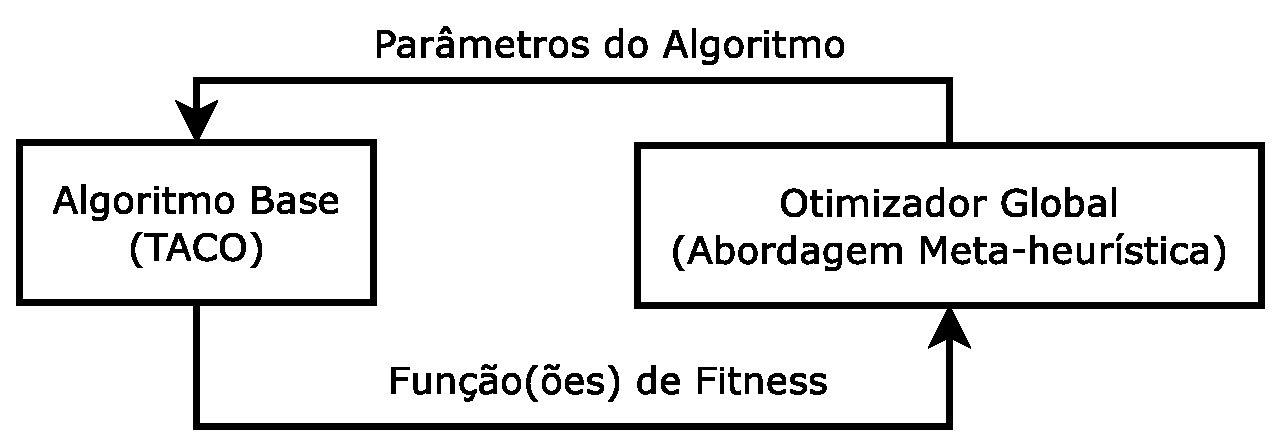
\includegraphics[width=0.75\textwidth]{imagens/proposal-diag.eps}
    \caption{Modelo de otimização associado a um otimizador global (OG)} \label{fig:proposal-diag}
\end{figure}

Conforme mostrado na Figura \ref{fig:proposal-diag}, o Otimizador Global (OG) começa a gerar um conjunto de valores para os parâmetros do TACO. Neste caso, os parâmetros otimizados do TACO são $\alpha$, $\beta$, $\xi$ e $\rho$. Então, a TACO constrói um conjunto de melhores soluções baseadas nos parâmetros otimizados. Em seguida, o TACO retorna ao OG o conjunto das melhores soluções, que são avaliadas para o algoritmo meta-heurístico. Conforme as iterações acontecem, o OG mantém um registro do melhor conjunto de parâmetros, que foram encontrados até o momento. A execução termina quando o OG atinge o limite de iterações.

% ---
\section{O Problema: distribuição de medicamentos}
\label{sec-metodologia-problema}
% ---

Uma CAF usualmente executa os pedidos de forma manual, tanto a separação da carga quanto o percurso estabelecido, independente do tempo gasto pelos entregadores. Devido à esta grande variação de tempo necessário no atendimento de pedidos, é difícil estabelecer uma capacidade para cada entregador, no intuito de mitigar os custos individuais dos percursos estabelecidos.

A metodologia deste trabalho consiste na criação de instâncias de MTSP a partir do ambiente real hospitalar e na aplicação de algoritmos baseados no ACO para a construção otimizada de soluções na distribuição de medicamento entre os entregadores.

Para este trabalho, foi desenvolvido uma instância MTSP tendo como base um hospital de grande porte, contendo farmácias satélites (FS) e uma CAF. Estas FSs estão distribuídas em diferentes blocos dentro do hospital e em diferente pavimentos. Na Figura \ref{fig:dataset-map} estão destacadas em preto as 16 farmácias em uma simulação para entregas durante o período diurno de um dia típico de trabalho. O ponto em vermelho está destacado a CAF, local onde os entregadores iniciam e concluem os seus percursos.

\begin{figure}[htb]
    \centering
    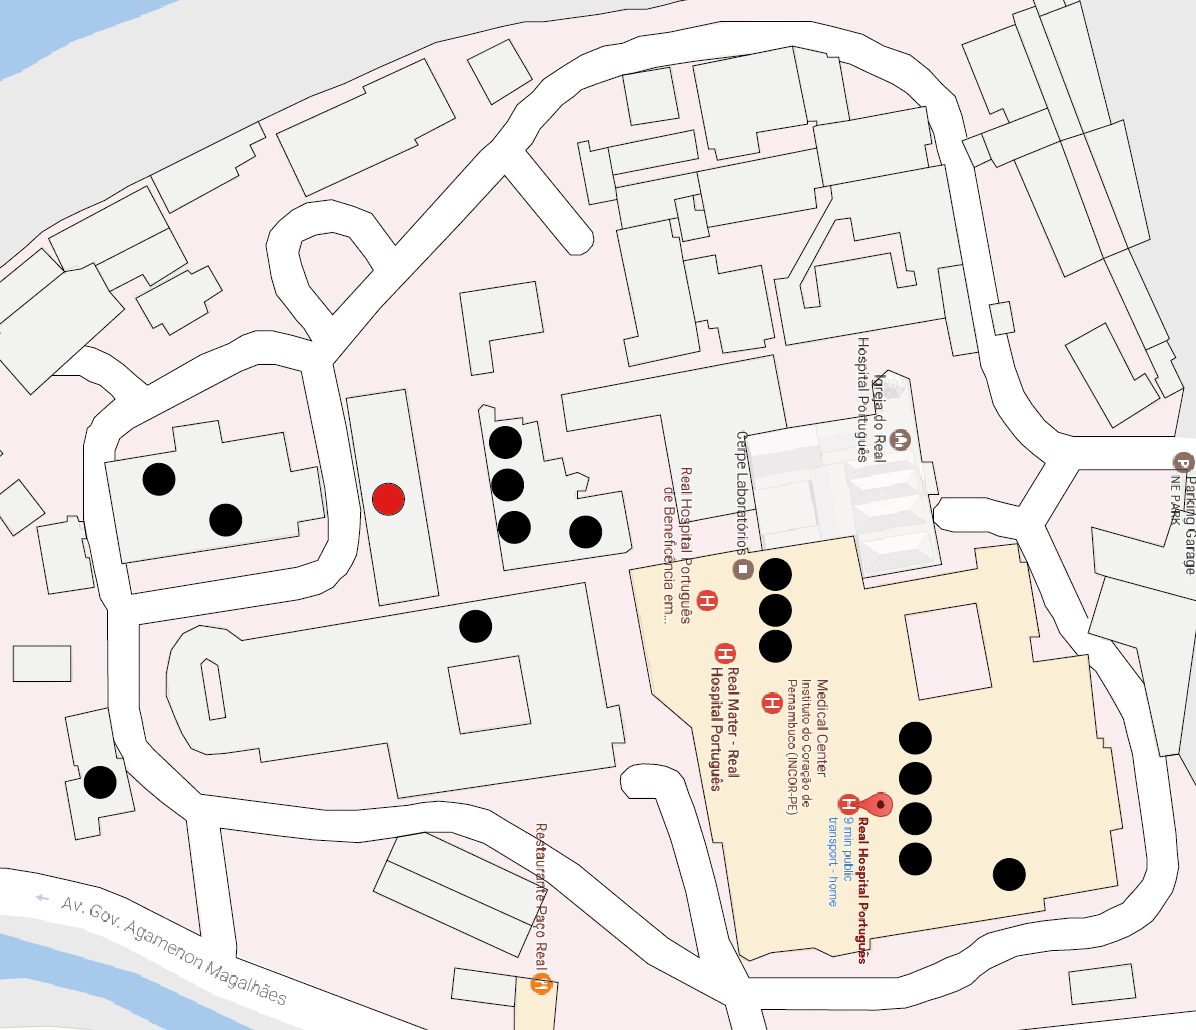
\includegraphics[width=0.75\textwidth]{imagens/dataset-map.png}
    \caption{Representação gráfica das farmácias e o CAF num grande hospital} \label{fig:dataset-map}
\end{figure}

Já na Figura \ref{fig:dataset-graph} mostra o grafo com os vértices representando cada farmácia satélite incluindo o centro de distribuição representado pelo vértice $X_0$, com os respectivos custos em suas arestas, cada mensageiro sai do vértice $X_0$, realiza a rota determinada pelo algoritmo e retorna para o centro de distribuição, $X_0$. Neste grafo há 17 nós (vértices) sendo cada nó $n$ é interligado aos outros $17 - n$ nós. Além disso, para esta abordagem, o problema é considerado como estático, isto é, todos os pedidos são feitos até as 8h da manhã pelas outras farmácias não considerando pedidos feitos depois do tempo limite.

\begin{figure}[htb]
    \centering
    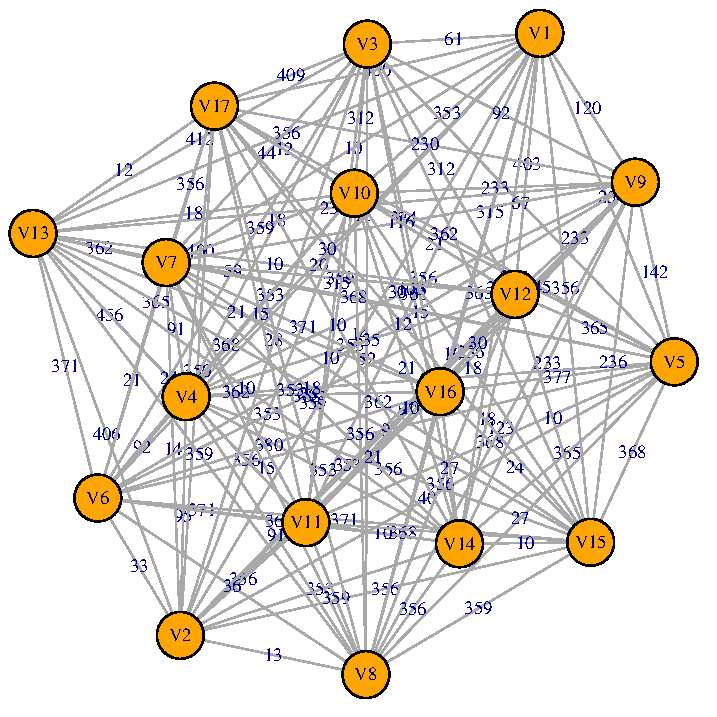
\includegraphics[width=0.75\textwidth]{imagens/dataset-graph.pdf}
    \caption{Modelo representado em forma de grafo com as suas arestas contendo as distâncias} \label{fig:dataset-graph}
\end{figure}

Uma matriz, chamada matriz de custo, contém os dados de cada farmácia, como número de registro ($id$), latitude, longitude e sua distância. A matriz ajuda a calcular o custo da rota. Da mesma forma, outra matriz, chamada de matriz de dados, contém as ordens de entrega para cada nó no modelo construído. Cada pedido contém registros do remetente e da farmácia, as distâncias iniciais e finais, quando o remetente deixou o CAF e a duração do pedido. A matriz de dados ajuda a simular um dia de pedido no depósito. Além disso, há quatro entregadores para entregar os pedidos às farmácias.

% ---
\section{Parâmetros a serem otimizados}
\label{sec-metodologia-parametros}
% ---

Como afirmado anteriormente, um otimizador global, baseado em inteligência de enxame, também é usado para melhorar os resultados do TACO, otimizando seus parâmetros. FSS, MOFSS e PSO são considerados como um otimizador global dos parâmetros TACO. Os valores padrão para o conjunto de parâmetros utilizados são: número de entregadores $M = 4$, número de equipes $N = 10$, probabilidade inicial $q_0 = 0,5$, relevância de feromônio $\alpha = 0,5$, relevância de visibilidade $\beta = 1,0$, persistência de feromônio para atualização local $\xi = 0,1$, persistência de feromônio para atualização global $\rho = 0,1$. Esses valores padrão foram obtidos por um teste de parâmetro. O critério de parada é de 1000 iterações para cada execução independente. Os otimizadores globais otimizam o subconjunto de parâmetros $P = \{\alpha, \beta, \xi, \rho\}$ em um intervalo de $0 \leq P \leq 2$.

% ---
\section{Metodologia Experimental}
\label{sec-metodologia-experimento}
% ---

Os experimentos apresentados nesta seção têm como objetivo mostrar a eficácia da metodologia desenvolvida aplicada ao problema real. No primeiro cenário, os algoritmos são configurados para minimizar o custo total das soluções, sem considerar a distribuição da carga de trabalho entre as equipes, como na descrição geral do MTSP. No segundo cenário, os algoritmos minimizam o custo da maior rota individual das soluções, visando a construção de soluções formadas por rotas com custos iguais entre os entregadores, como no MTSP com balanceamento de carga de trabalho.

% ---
\subsection{Ambiente de Simulação}
\label{subsec-metodologia-experimento}
% ---

Todos os experimentos foram executados em um MacBook Pro (13 polegadas, final de 2011) com CPU Intel Core i5 de 2,4 GHz, 16 GB de RAM (1333 MHz DDR3) e sistema operacional MacOS High Sierra (versão 10.13.4). Usamos o banco de dados apresentado na Seção \ref{sec-metodologia-problema}. Em seguida, realizamos 30 execuções independentes dos algoritmos para cada experimento. O algoritmo TACO foi codificado em Java com base no algoritmo proposto por Valivaara (2007). O FSS é baseado na versão de Verçosa, Bastos-Filho e Monteiro (2017) \cite{verccosa2017combining}. O PSO de objetivo único foi retirado da estrutura do jMetal (DURILLO; NEBRO, 2011) \cite{durillo2011jmetal}. O MOFSS utilizado é baseado na versão de Bastos-Filho e Guimarães (2015) \cite{bastos2015multi} utilizando o jMetal como framework para visualizações.

O TACO desenvolvido por Valivaara foi utilizado por ter apresentado bons resultados na resolução de problemas do tipo MTSP durante experimentos prévios no desenvolvimento deste trabalho. O algoritmo foi codificado em Java para facilitar a integração com outras ferramentas já disponíveis e algoritmos utilizados como OGs. Já o FSS desenvolvido foi escolhido Verçosa, Bastos-Filho e Monteiro por ter como base a versão FSS Vanilla (disponível em \url{http://www.fbln.pro.br/fss/versions.htm}) e apresentar estruturação das classes compatível com os problemas da Conference on Commerce and Enterprise Computing (CEC). 

O jMetal é um repositório criado por Durillo et al. em 2010, e que utiliza linguagem de programação Java, e fornece a implementação de vários algoritmos existentes na literatura, tanto mono quanto multi-objetivo. A utilização desta ferramenta contribuiu, de forma significativa, no auxilio do desenvolvimento deste trabalho, visto que algumas necessidades já estavam implementadas, poupando tempo de desenvolvimento. Além disso, o PSO utilizado neste trabalho provem deste framework cuja a implementação corresponde ao PSO padrão.

Por fim, O MOFSS baseado na versão de Bastos-Filho e Guimarães foi escolhido por ter sido desenvolvido utilizando o framework JMetal o que facilita na integração com os outros algoritmos desenvolvidos em Java. Além disso, esta implementação gera gráficos dos operadores utilizados pelo MOFSS e o gráfico contendo as soluções não-dominadas.

% ---
\subsection{Métrica de Avaliação}
\label{sec-metodologia-experimento}
% ---

A comparação de desempenho de um ou vários métodos de otimização mono e multi-objetivo requer parâmetros que possam ser relacionados e comparáveis. Neste trabalho, a métrica utilizada foi o desvio padrão (DP) calculado em cima da média de resultados de 30 simulações independentes. O DP é um parâmetro muito usado em estatística que indica o grau de variação de um conjunto de elementos, i.e., é uma medida que expressa o grau de dispersão de um conjunto de dados. Logo, o desvio padrão indica o quanto um conjunto de dados é uniforme. Quanto mais próximo de 0 for o desvio padrão, mais homogêneo são os dados.

% ---
\subsection{Configuração dos experimentos}
\label{sec-metodologia-config}
% ---

O TACO participa do experimento como um algoritmo de base. Antes de iniciar os experimentos do modelo proposto, um teste de base deve ser realizado para comprovar a eficácia e robustez do algoritmo escolhido. Os valores padrão para ambos os cenários são indicados na Seção \ref{sec-metodologia-parametros}. O FSS como um GO é executado com um critério de parada de 1000 iterações por execução e possui 30 execuções independentes. Os valores dos parâmetros do FSS foram retirados do trabalho de Verçosa, Bastos-Filho e Monteiro (2017). Da mesma forma, o PSO tem os mesmos valores de critério de parada e execuções independentes. Os valores do parâmetro PSO permaneceram os mesmos que no framework jMetal. Por fim, foram mantidos os valores padrões apresentados no trabalho de Bastos-Filho e Guimarães para a abordagem MOFSS.
\chapter{Resultados}

%\lipsum[1-1]

%POR QUE O PROBLEMA DA MOCHILA NÃO ENTROU?
%FAÇA COMPARAÇÃO COM FORÇA-BRUTA! UM DAS SOLUÇÕES APRESENTADAS DEMORA QUASE 5 HORAS!!!
O primeiro conjunto de experimentos foi realizado para minimizar o Custo Total de Rotas (CTR), ou seja, a soma da rota de cada equipe. Ao comparar as soluções, que possui o menor custo total, é considerada a melhor. Este cenário pode ser aplicado à vida real quando pretendemos reduzir a quantidade total de rotas de entrega em vez de priorizar o equilíbrio de trabalho.

O segundo conjunto de experimentos visou minimizar a Rota Mais Longa (RML) das soluções mantendo os mesmos valores dos parâmetros no primeiro cenário. Esse caso é adequado para situações reais quando priorizamos o equilíbrio entre as rotas individuais (\textit{workbalance}) em vez da soma total das rotas.

Os resultados mostrados aqui são referentes ao experimentos somente envolvendo o MTSP (\textit{Multiple Travelling Salesmen Problem}). O tratamento subsequente para soluções envolvendo tanto o MTSP quanto KP (\textit{Knapsack Problem}) não foi tratado nestes experimento devido a ajustes que entrarão na continuação deste trabalho.

% ---
\section{Resultados sem Otimizadores Globais}
\label{sec-resultados-taco}
% ---

Foi utilizado a abordagem TACO com regras do ACS para otimização da instância vista na Seção 5 para quatro entregadores. Foram realizados dois experimentos: minimização do custo total das soluções e minimização da maior rota individual das soluções.

A Tabela \ref{tab:resultado-taco} mostra a distância média de execução do algoritmo (em quilômetros) para a instância. Este valor foi obtido a partir da média da distância encontrada (tanto para Custo Total de Rotas - CTR quanto para Rota Mais Longa - RML) nos 1000 ciclos TACO e nas 30 execuções do algoritmo, por um dia útil. Os resultados provam a robustez dao algoritmo é minimizar os resultados para CTR e RML.

\begin{table}[htb]
    \centering
    \caption{Resultados para o TACO sem Otimizadores Globais} \label{tab:resultado-taco}
\begin{tabular}{|c|c|c|c|c|c|c|c|}
\hline
\multicolumn{8}{|c|}{Média de 30 simulações com 1000 iterações}                                                            \\ \hline
\multicolumn{4}{|c|}{Minimizando o Custo Total das Rotas (CTR)} & \multicolumn{4}{c|}{Minimizando a Rota Mais Longa (RML)} \\ \hline
CTR (km)    & D.P.  & RML (km)  & D.P.      & CTR (km)  & P.D.      & RML (km)  & D.P.        \\ \hline
1,8         & 0,25  & 0,721     & 0,003     & 1,223     & 0,050     & 0,756     & 0,012       \\ \hline
\end{tabular}
\end{table}

O TACO apresentou resultados satisfatórios para as duas variações do MTSP: minimizar o custo total da solução e minimizar o custo da maior rota de solução individual (Tabela \ref{tab:resultado-taco}). Os pequenos valores dos desvios padrão nas duas tabelas confirmam a robustez do algoritmo ao gerar soluções com custos próximos da média das 30 execuções. Embora a RL esteja sendo minimizada, o TCR varia ao longo das iterações, conforme observado no Figura \ref{fig:resultados-convergencia-taco-tcr}. A mesma situação ocorre quando a TACO minimiza o TCR (ver Figura \ref{fig:resultados-convergencia-taco-rml}). Tendo isso em mente, ainda há espaço para melhorias nos resultados de ambos os objetivos.

\begin{figure}[htb]
    \centering
    \caption{Curva de convergência quando minimizado o CTR} \label{fig:resultados-convergencia-taco-tcr}
    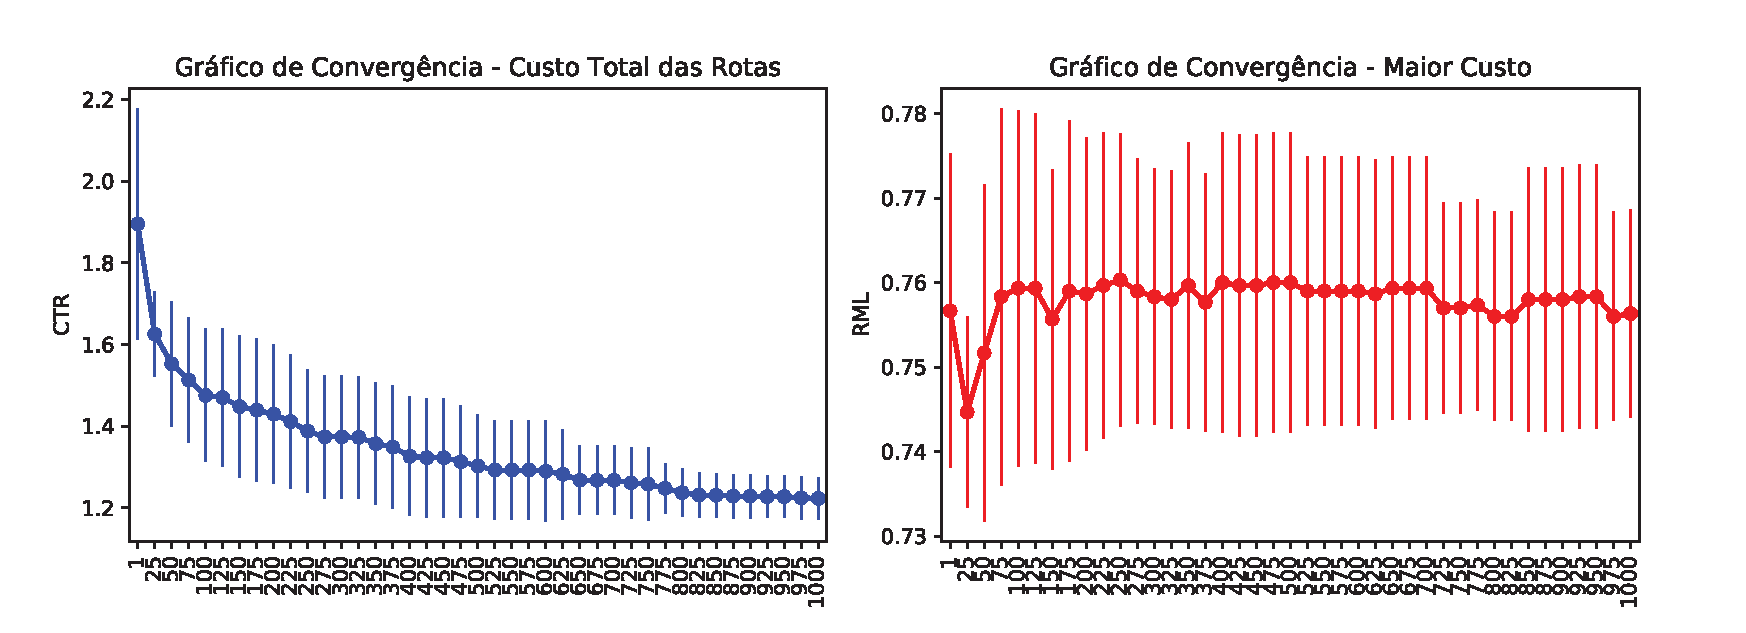
\includegraphics[width=\textwidth]{imagens/convergence-totalcost-taco.eps}
    \end{figure}

\begin{figure}[htb]
    \centering
    \caption{Curva de convergência quando minimizado RML} \label{fig:resultados-convergencia-taco-rml}
    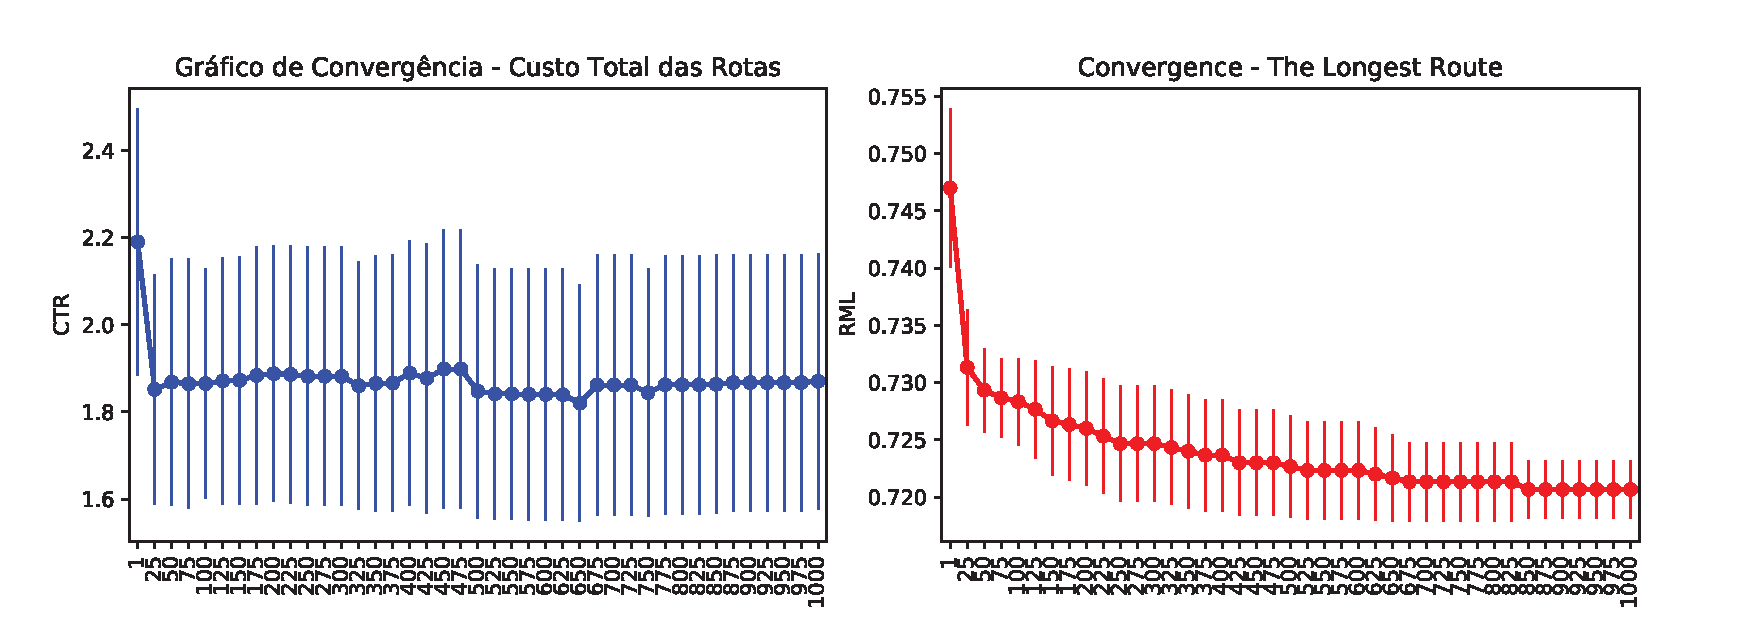
\includegraphics[width=\textwidth]{imagens/convergence-maxcost-taco.eps}
\end{figure}

% ---
\section{Resultados com Otimizadores Globais}
\label{sec-resultados-fss-pso}
% ---

Os experimentos realizados com o otimizador externo mostraram melhores resultados para ambos os cenários, mostrados nas Tabelas \ref{tab:resultado-fsstaco} e \ref{tab:resultado-psotaco}. Comparando as Tabelas \ref{tab:resultado-taco} e \ref{tab:resultado-fsstaco}, o FSS tem uma melhora melhor ao minimizar a rota mais longa em comparação ao algoritmo base. Esse resultado é devido à capacidade do FSS de explorar o espaço de pesquisa. Além disso, o FSS apresenta um desvio padrão menor, o que corrobora a sua robustez.

\begin{table}[htb]
    \centering
    \caption{Resultados para TACO com FSS sendo o Otimizador Global} \label{tab:resultado-fsstaco}
\begin{tabular}{|c|c|c|c|c|c|c|c|}
\hline
\multicolumn{8}{|c|}{Média de 30 simulações com 1000 iterações}                                                            \\ \hline
\multicolumn{4}{|c|}{Minimizando o Custo Total das Rotas (CTR)} & \multicolumn{4}{c|}{Minimizando a Rota Mais Longa (RML)} \\ \hline
CTR (km)    & D.P.   & RML (km)  & D.P.  & CTR (km)  & D.P.     & RML (km)  & D.P.        \\ \hline
1,0797      & 0,002  & 0,747     & 0     & 1,944     & 0,335    & 0,719     & 0,001       \\ \hline
\end{tabular}
\end{table}

\begin{figure}[htb]
    \centering
    \caption{Curva de convergência FSS-TACO quando minimizado o CTR} \label{fig:resultados-convergencia-fss-tcr}
    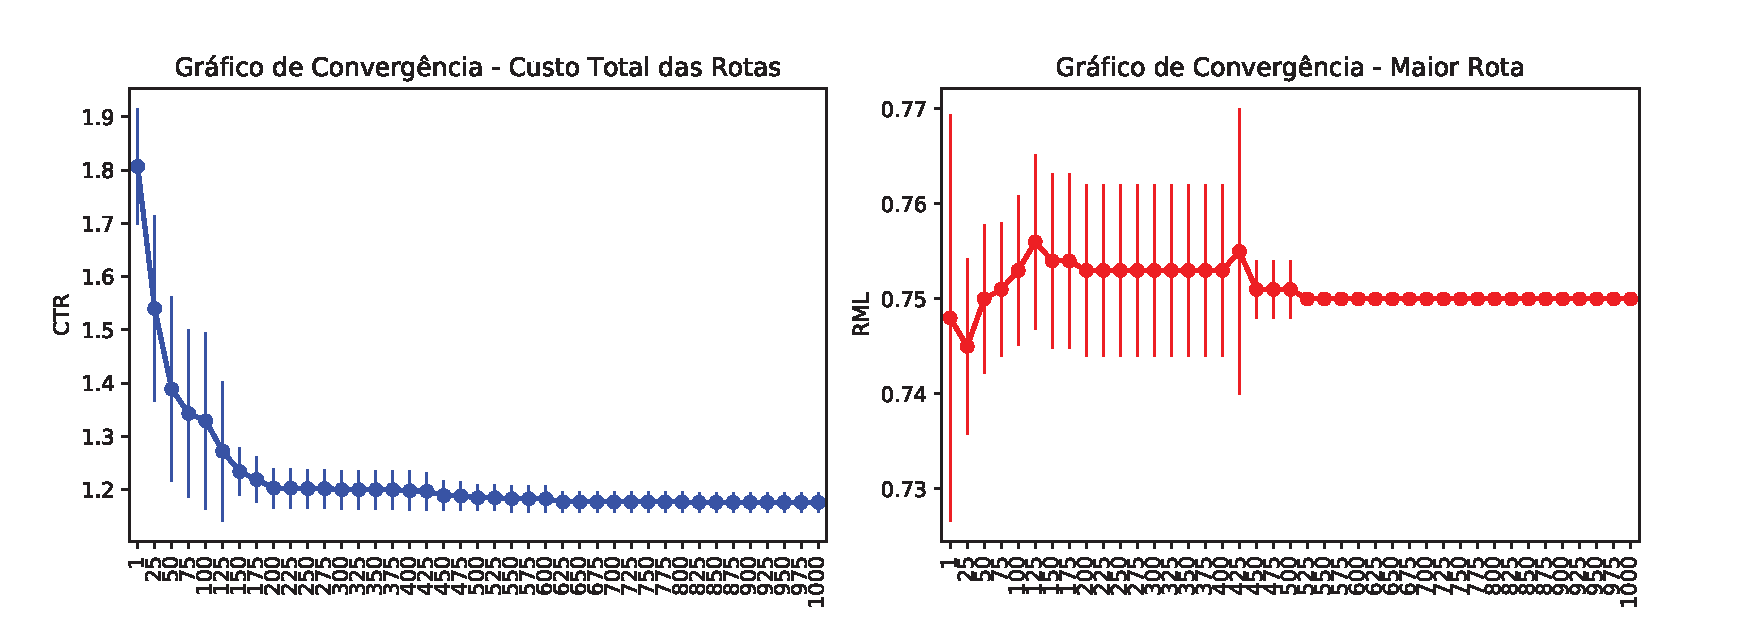
\includegraphics[width=\textwidth]{imagens/convergence-totalcost-fsstaco.eps}
\end{figure}

\begin{figure}[htb]
    \centering
    \caption{Curva de convergência FSS-TACO quando minimizado a RML} \label{fig:resultados-convergencia-fss-rml}
    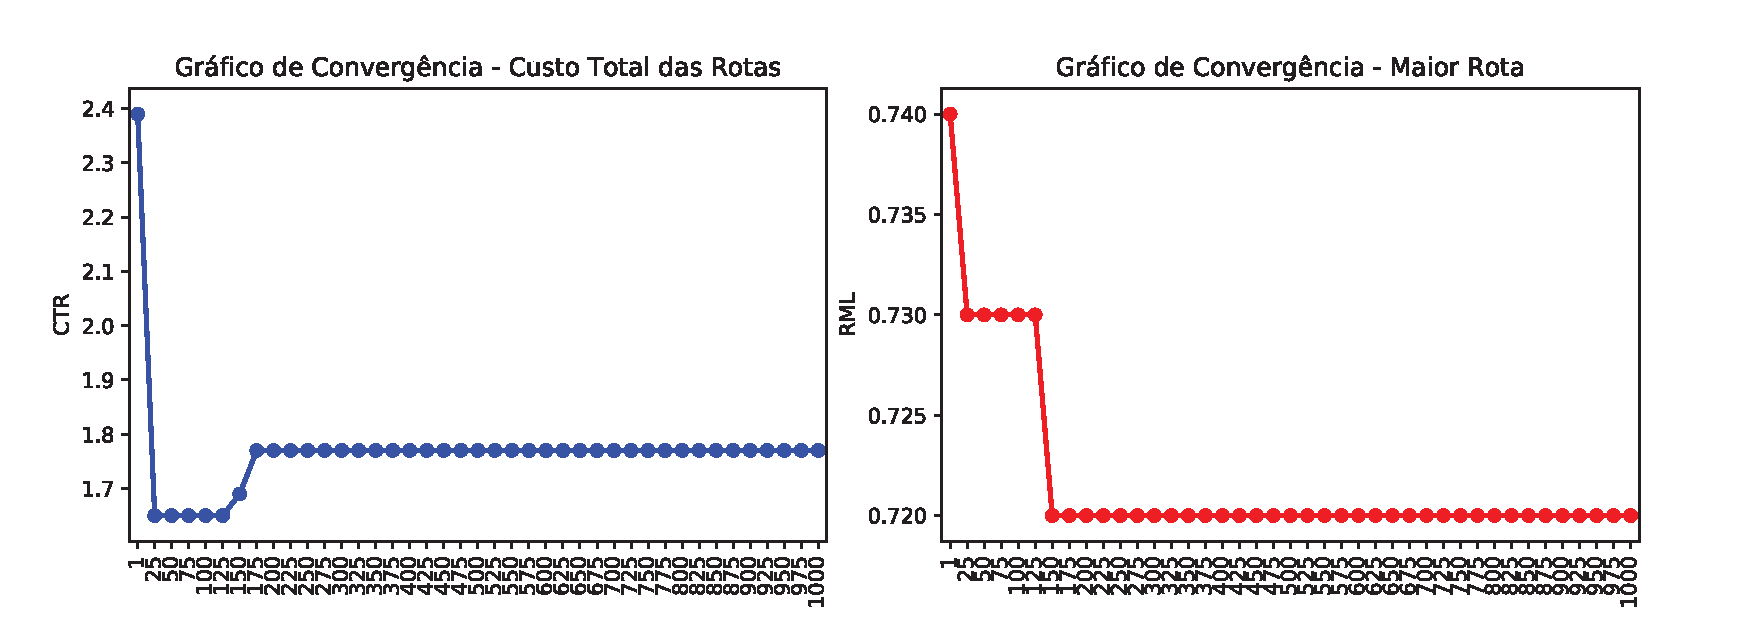
\includegraphics[width=\textwidth]{imagens/convergence-maxcost-fsstaco.eps}
\end{figure}

PSO também teve melhores resultados em comparação com abordagem TACO sem otimizadores externos (ver Tabela \ref{tab:resultado-psotaco}). Seu desvio padrão também mostra a robustez e eficácia ao otimizar TCR e LR.

\begin{table}[htb]
    \centering
    \caption{Resultados para TACO com PSO sendo o Otimizador Global} \label{tab:resultado-psotaco}
\begin{tabular}{|c|c|c|c|c|c|c|c|}
\hline
\multicolumn{8}{|c|}{Média de 30 simulações com 1000 iterações}                                                            \\ \hline
\multicolumn{4}{|c|}{Minimizando o Custo Total das Rotas (CTR)} & \multicolumn{4}{c|}{Minimizando a Rota Mais Longa (RML)} \\ \hline
CTR (km)    & D.P.   & RML (km)  & D.P.   & CTR (km)  & D.P.     & RML (km)  & D.P.        \\ \hline
1,115       & 0,032  & 0,750     & 0,003  & 2,048     & 0,333    & 0,720     & 0,005       \\ \hline
\end{tabular}
\end{table}

\begin{figure}[htb]
    \centering
    \caption{Curva de convergência PSO-TACO quando minimizado o CTR} \label{fig:resultados-convergencia-pso-tcr}
    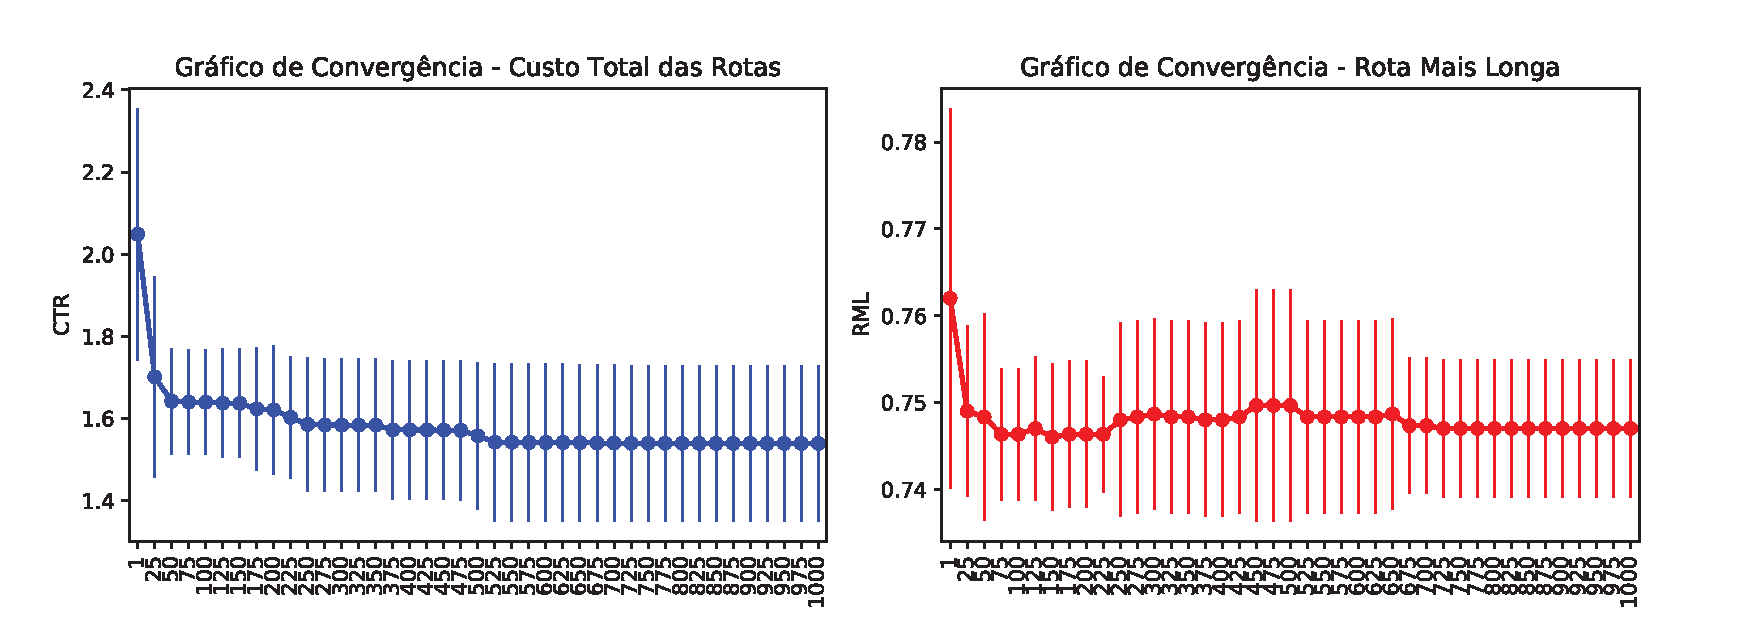
\includegraphics[width=\textwidth]{imagens/convergence-totalcost-psotaco.eps}
\end{figure}

\begin{figure}[htb]
    \centering
    \caption{Curva de convergência PSO-TACO quando minimizado a RML} \label{fig:resultados-convergencia-pso-rml}
    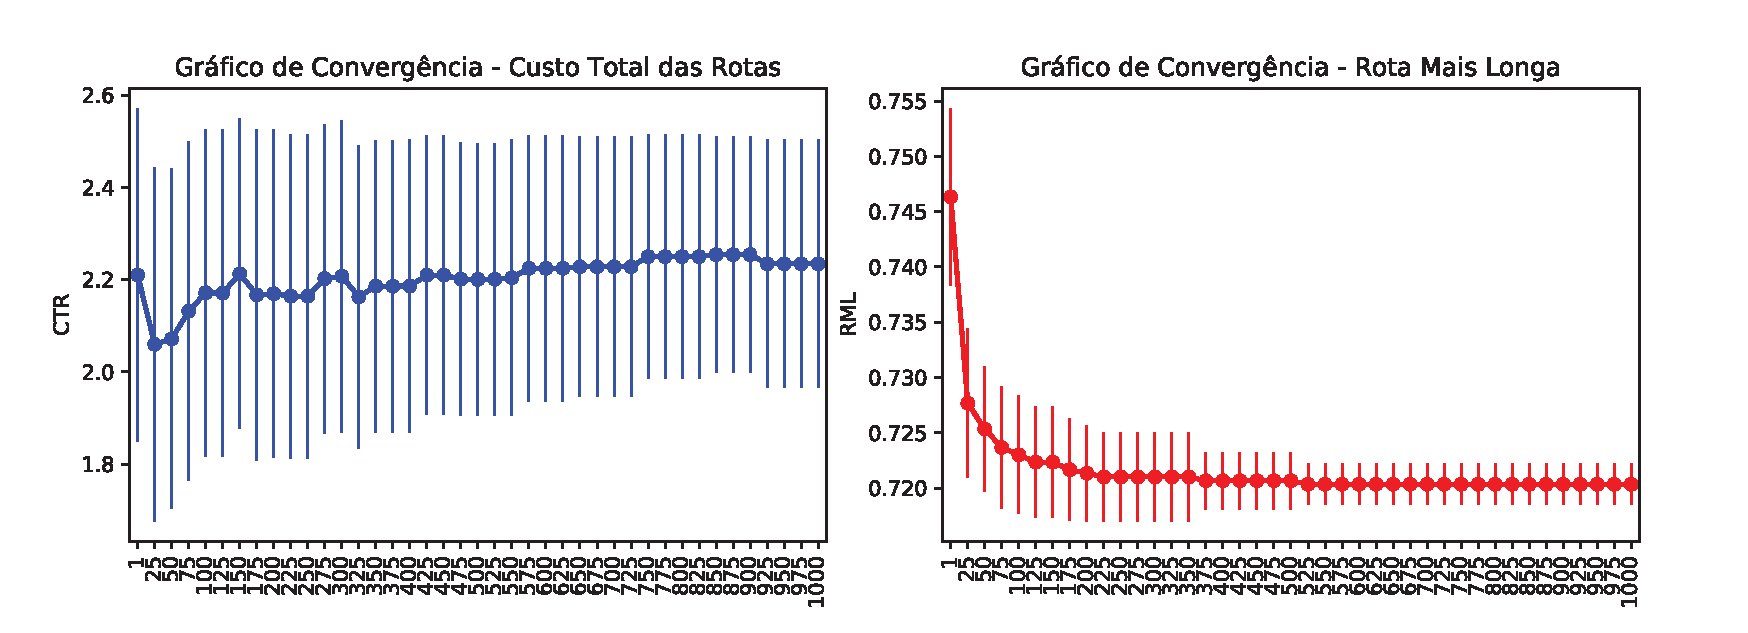
\includegraphics[width=\textwidth]{imagens/convergence-maxcost-psotaco.eps}
\end{figure}

Os experimentos realizados com o otimizador externo mostraram melhores resultados para ambos os cenários, mostrados nas Tabelas \ref{tab:resultado-fsstaco} e \ref{tab:resultado-psotaco}. Conforme apresentado nas Tabelas \ref{tab:resultado-taco} e \ref{tab:resultado-fsstaco}, o FSS tem uma melhora melhor de minimizar a rota mais longa em comparação ao algoritmo base. Esse resultado é devido à capacidade do FSS de explorar o espaço de pesquisa. Além disso, o FSS apresenta um desvio padrão menor, o que corrobora sua robustez.

% ---
\section{Comparativo entre os experimentos}
\label{sec-resultados-taco}
% ---

Todos os resultados anteriores são compilados na Tabela \ref{tab:resultado-comparison} para um melhor entendimento. Comparando as três abordagens, o FSS obteve melhores resultados ao minimizar tanto o CTR quanto a RML. Também teve o menor resultado com um desvio padrão próximo de zero. Como visto na Figura \ref{fig:resultados-convergencia}, em ambos os cenários, o FSS convergiu mais cedo do que o PSO e o algoritmo de base. Os resultados do PSO foram melhores que os resultados do algoritmo de base e convergiram mais cedo do que o TACO como esperado.

\begin{figure}[htb]
    \centering
    \caption{Comparação entre as convergências de TACO, FSS-TACO e PSO-TACO} \label{fig:resultados-convergencia}
    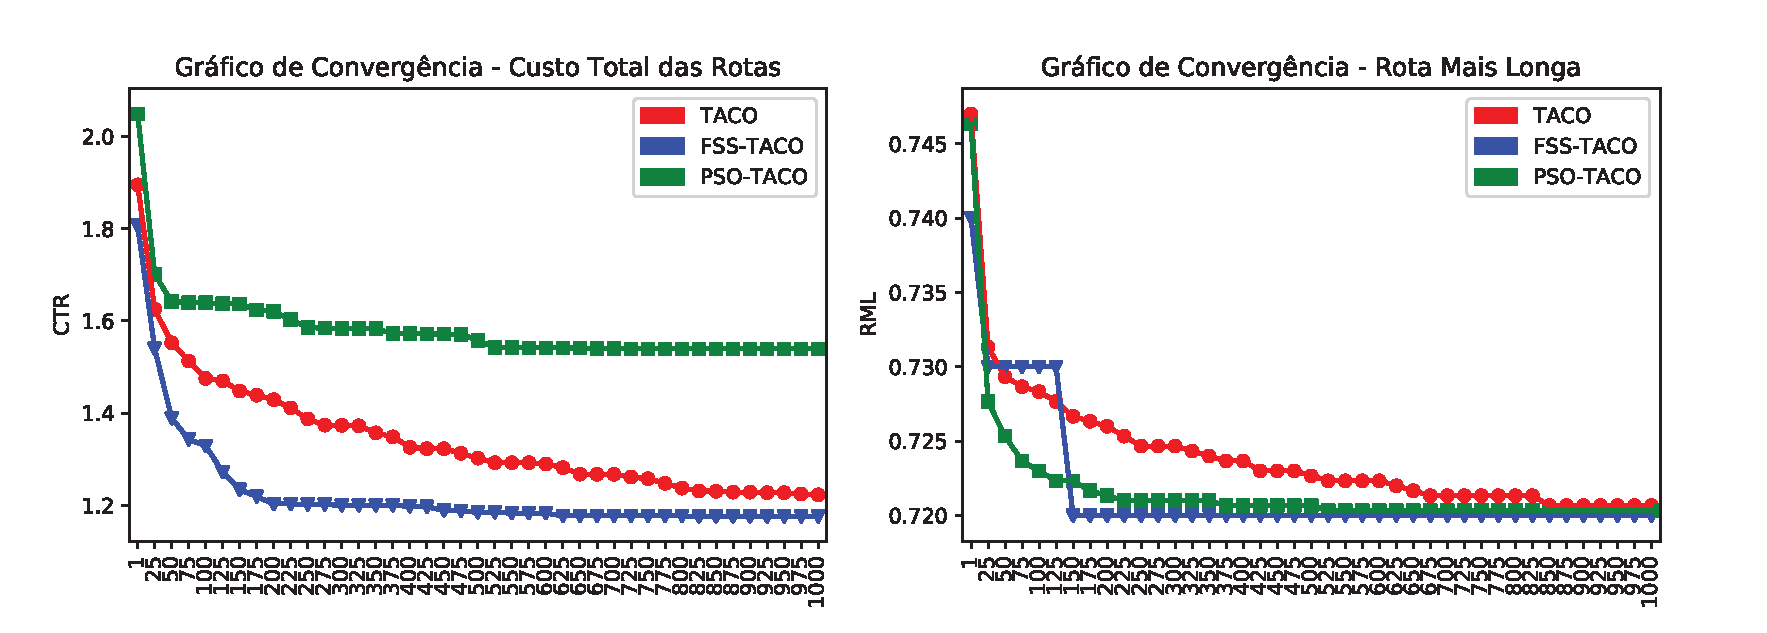
\includegraphics[width=\textwidth]{imagens/convergence-approaches.eps}
\end{figure}

% Please add the following required packages to your document preamble:
% \usepackage{multirow}
\begin{table}[htb]
    \centering
    \caption{Comparação entre resultados com 30 simulações independentes} \label{tab:resultado-comparison}
\begin{tabular}{|c|c|c|c|c|c|c|c|c|}
\hline
\multirow{2}{*}{Abordagem} & \multicolumn{4}{l|}{Minimizando o CTR}           & \multicolumn{4}{l|}{Minimizando a RML}          \\ \cline{2-9} 
                            & CTR (km)             & D.P.           & RML (km)   & D.P.  & CTR (km)   & D.P.  & RML (km)            & D.P.           \\ \hline
TACO                       & 1,8             & 0,25           & 0,721 & 0,003 & 1,223 & 0,050 & 0,756          & 0,012          \\ \hline
FSS-TACO                   & \textbf{1.0797} & \textbf{0.002} & 0,747 & 0     & 1,944 & 0,335 & \textbf{0.719} & \textbf{0.001} \\ \hline
PSO-TACO                   & 1,115           & 0,032          & 0,750 & 0,003 & 2,048 & 0,333 & 0,720          & 0,005          \\ \hline
\end{tabular}
\end{table}

A Figura \ref{fig:resultados-boxplot} mostra o desvio padrão para ambos os CTR e RML. Ao minimizar o CTR, podemos notar que os resultados do TACO variam mais do que o FSS e PSO. Por outro lado, PSO tem a menor variação de seus resultados. Ao minimizar a RML, vale ressaltar que para todas as abordagens (TACO, FSS e PSO) existe uma pequena ou nenhuma variação entre seus resultados.

\begin{figure}[!htb]
    \centering
    \caption{Boxplot com os desvios padrões da minimização do CTR e da RML} \label{fig:resultados-boxplot}
    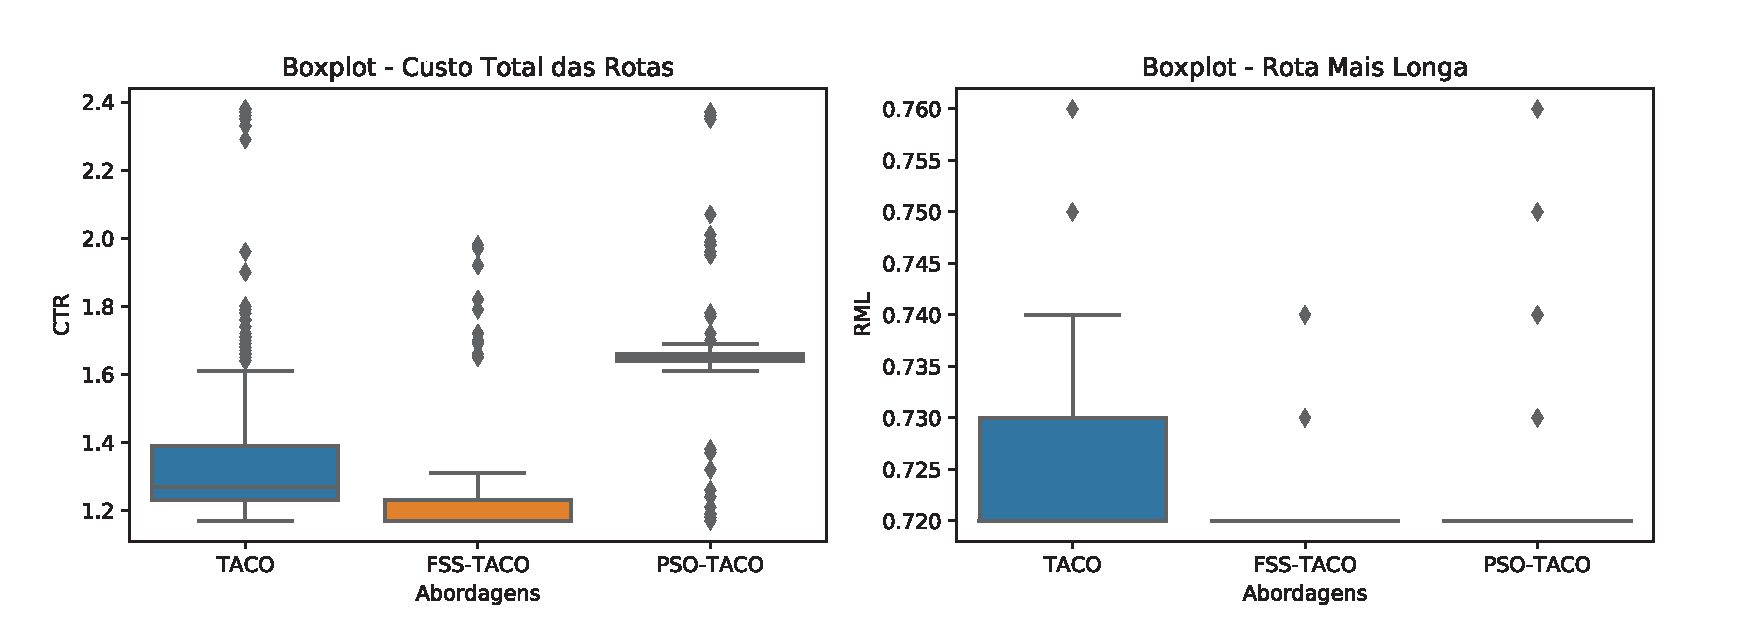
\includegraphics[width=\textwidth]{imagens/boxplot-approaches.eps}
\end{figure}

% ---
\section{Tempos de Execução dos Algoritmos}
\label{sec-resultados-tempo}
% ---

A Tabela \ref{tab:resultado-tempo} apresenta o tempo médio de execução do algoritmo para cada instância. Este valor foi obtido a partir da média do tempo (em milissegundos) gasto para execução dos 1000 ciclos de cada abordagem nas 30 execuções independente do algoritmo.

% Please add the following required packages to your document preamble:
% \usepackage{multirow}
\begin{table}[htb]
    \centering
    \caption{Tempo médio de execução de 1.000 ciclos de TACO, FSS-TACO e PSO-TACO} \label{tab:resultado-tempo}
    \begin{tabular}{|c|c|c|c|c|}
    \hline
    \multirow{2}{*}{Abordagem} & \multicolumn{2}{c|}{Minimizando o CTR} & \multicolumn{2}{c|}{Minimizando a RML}          \\ \cline{2-5} 
                               & Média em ms & Média em horas  & Média em ms & Média em horas  \\ \hline
    %TACO                       & 618,53     &T       & 609,73 &T            \\ \hline
    TACO                       & $6,185 \times 10^2$     &$0,017 \times 10^{-2}$       & $6,097 \times 10^2$ &$0,0169 \times 10^{-2}$            \\ \hline
    %FSS-TACO                   & 16.945.914,10  &T     & 15.701.984,33 &T      \\ \hline
    FSS-TACO                   & $1,695 \times 10^7$  &4,707     & $1,570 \times 10^7$ &4,362      \\ \hline
    %PSO-TACO                   & 5.218.562,20   &T     & 5.161.234,17    &T    \\ \hline
    PSO-TACO                   & $5,21856220 \times 10^6$  &1,450     & $5,161 \times 10^6$    &1,434    \\ \hline
    \end{tabular}
\end{table}

Quanto aos tempos de execução do algoritmo, mostrados na Tabela \ref{tab:resultado-tempo}, verifica-se que para a instância experimentada, foram gastos em media aproximadamente 0,6 segundo para execução dos 1000 ciclos do algoritmo, que representam um tempo aceitável para o problema em estudo. Entretanto, ao comparar a abordagem utilizando os OGs PSO e FSS o tempo médio de execução passa 1 hora e 4 horas, respectivamente. Em ambos os cenários de otimização (minimizando CTR ou RML), a abordagem com OG sendo PSO é mais rápida do que o OG sendo o FSS. Ao levar em consideração o tempo que os pedidos são feitos ao CAF (pedidos aceitos até às 8h da manhã), o PSO leva vantagem pois o tempo de processamento é menor, levando a um menor tempo na distribuição dos medicamentos.

% ---
\section{Análise dos Resultados o MOFSS-TACO}
\label{sec-resultados-tempo}
% ---

%COLOCAR OS RESULTADOS FINAIS DO MOFSS-TACO
Os resultados para o MOFSS sendo o OG do algoritmo base (ver Tabela \ref{tab:resultado-mofss}) se mostram bastante interessantes. Ao minimizar simultaneamente CTR e RML, o MOFSS consegue resultados menores que o TACO sem otimizador externo, tendo em vista os valores otimizados do TACO de forma mono-objetiva como visto na Tabela \ref{tab:resultado-taco}. Entretanto, para os resultados parciais não são menores quando comparados as abordagens PSO-TACO e FSS-TACO. Todavia, deve ser levado em consideração que os objetivos CTR e RML estão sendo minimizados de forma simultânea o que garante um tempo de execução menor dos que os outros dois.

\begin{table}[htb]
    \centering
    \caption{Resultados para TACO com MOFSS sendo o Otimizador Global} \label{tab:resultado-mofss}
    \begin{tabular}{|c|c|c|c|}
    \hline
    \multicolumn{4}{|c|}{Média de 30 simulações com 1000 iterações} \\ \hline
    \multicolumn{4}{|c|}{Minimizando CTR e RML}                     \\ \hline
    CTR            & D.P.          & RML            & D.P.          \\ \hline
    1,398          & 0,279         & 0,732          & 0,011         \\ \hline
    \end{tabular}
    \end{table}

Ao fim de cada execução, a abordagem MOFSS-TACO gera um conjunto de soluções ótimas não-dominadas. Como o problema não tem grande complexidade, ao final de cada execução independente gera um conjunto com quatro soluções não dominadas.

\section{Discussão dos Resultados}

O resultado do desvio padrão (D.P.) se mostra satisfatório confirmando a robustez do algoritmo para os experimentos contemplando somete o TACO. Comparado com a minimização dos dois objetivos, a minimização da RML foi inferior na minimização do CTR. Essa otimização proporciona um número maior de entregas pelos entregadores visto que o custo da rota individual é balanceado de modo a não sobrecarregar ou ocasionar ociosidade em um dos entregadores. Com os entregadores realizando mais entregas em menos tempo, essa técnica é mais favorável quando o custo total do deslocamento não é o objetivo, mas sim a quantidade de entregas por cada entregador.

Vale ressaltar que, na minimização do CTR, a carga não é distribuída de maneira uniforme para os entregadores podendo um ou mais entregadores ficar com sobrecarga ou ocioso dependendo da configuração. Já na minimização da RML, focado em minimizar a maior rota individual, distribuindo a carga de maneira uniforme para todos os entregadores.

Ao comparar os resultados, sem e com OGs e otimização mono-objetivo, é possível perceber o bom desempenho da abordagem FSS-TACO em face das abordagens TACO e PSO-TACO. Entretanto, o seu uso se torna inviável, dependendo da situação, por requerer um tempo de execução superior aos das outras abordagens presentes na comparação. Para uma abordagem multi-objetiva, o MOFSS sendo o OG do algoritmo base, mostra resultados parciais interessantes visto que obteve resultados melhores para CTR e RML se comparado aos resultados do algoritmo base. Como a instância construída para este trabalho não possui grande complexidade, a Curva de Pareto, com as soluções ótimas, se restringe a quatro soluções não-dominadas.
\chapter{Conclusão}

%\lipsum[1-1]

\section{Conclusão}

O problema de Múltiplos Caixeiros Viajantes (MTSP) vem sendo estudado nas últimas duas décadas apresentando várias abordagens para a otimização de suas soluções. Entretanto, ainda é escasso estudos relacionados ao MTSP dentro da área hospitalar. Este trabalho mostra que a distribuição de medicamentos em um hospital de grande porte ou em grande rede de farmácias pode ser realizada de forma eficiente com o auxílio de uma ferramenta computacional.

O modelo proposto descrito foi eficiente na distribuição das ordens de serviço entre os entregadores e na criação de rotas otimizadas para a realização dos serviços. No entanto, algumas questões precisam ser analisadas, como a otimização multi-objetivo do custo total das rotas e a rota mais longa e a otimização das mochilas dos entregadores.

Para a criação de soluções otimizadas para MTSP neste trabalho, um algoritmo baseado na meta-heurística ACO foi implementado e associado a um otimizador global. O FSS e PSO foram responsáveis por otimizar os parâmetros TACO para melhorar os resultados.

Como mostrado na Seção 6, o FSS alcançou os melhores resultados para ambos os cenários, com os menores resultados de minimização para o Custo Total de Rotas (CTR) e a Rota Mais Longa (RML) com desvios padrão em torno de zero. Nesses dois casos, o FSS como otimizador global convergiu mais cedo do que as outras duas abordagens.

Outra abordagem possível para o problema do MTSP é otimizar os dois objetivos simultaneamente, CTR e RML. Para atingir este objetivo, foi utilizando um algoritmo de otimização multi-objetivo chamado Multi-Objective Fish School Search (MOFSS). Os resultados parciais mostram um bom desempenho em relação ao algoritmo base (TACO). Ao minimizar CTR RML concomitantemente, a abordagem mostra melhores resultados se comparado ao TACO sem utilização de otimizadores externos. Para o problema do mundo real, é imprescindível este tipo de abordagem para que se possa fazer a mitigação de perdas e custos no processo de distribuição bem como otimizar o capital humano dispendido nos processos de logística.

\section{Trabalhos Futuros}

Como trabalho futuro, pretende-se verificar a utilização de algumas variações de valores para os operadores dos otimizadores globais a fim de encontrar melhores configurações. Também deve ser verifcado a distribuição dos medicamentos reduzindo variando o quadro de entregadores (aqui considerados como caixeiros da instância MTSP).

Outra meta-heurística que tem obtido resultados consistentes para problemas de otimização combinatória são os Algoritmos Genéticos (AG) \cite{somhom1999competition}, que serão utilizados como otimizadores globais para comparação com os resultados obtidos pelos experimentos deste trabalho em novos experimentos.

Para análise e efeito comparativo entre a proposta e os algoritmos de estado-da-arte, pretende-se realizar testes estásticos com os dados coletados durante as simulações da instância MTSP criada para a verificação de desempenho. Experimentos com a proposta e abordagens multi-objetivas como SMPSO (NEBRO et al., 2009) \cite{nebro2009}, MOEA/D (ZHANG; LI, 2007) \cite{zhang2007} e SPEA2 (ZITZLER; LAUMANNS; THIELE, 2001) \cite{zitzler2001} também serão realizados para verificar a robustez e eficiência. Como consequência, haverá realização de um quadro comparativo entre as diferentes instâncias do problema e a aplicação das abordagens citadas neste trabalho.

Por último, outro ponto diz respeito ao caráter dinâmico do ambiente em estudo. Enquanto a metodologia proposta mostra-se viável para cenários estáticos, no qual todas as ordens e as posições dos entregadores são conhecidas antes da otimização, no ambiente real serviços surgem durante o dia de trabalho dos entregadores e podem ter maior prioridade que outros, como as ordens emergenciais. Para tratamento desta demanda, a metodologia desenvolvida será adaptada para gerar novas soluções otimizadas a cada mudança no ambiente real, como o surgimento de novas ordens.
% \chapter{Resultados de comandos}\label{cap_exemplos}

% ---
\section{Codificação dos arquivos: UTF8}
% ---

A codificação de todos os arquivos do \abnTeX\ é \texttt{UTF8}. É necessário que
você utilize a mesma codificação nos documentos que escrever, inclusive nos
arquivos de base bibliográficas |.bib|.

% ---
\section{Citações diretas}
\label{sec-citacao}
% ---

\index{citações!diretas}Utilize o ambiente \texttt{citacao} para incluir
citações diretas com mais de três linhas:

\begin{citacao}
As citações diretas, no texto, com mais de três linhas, devem ser
destacadas com recuo de 4 cm da margem esquerda, com letra menor que a do texto
utilizado e sem as aspas. No caso de documentos datilografados, deve-se
observar apenas o recuo \cite[5.3]{NBR10520:2002}.
\end{citacao}

Use o ambiente assim:

\begin{verbatim}
\begin{citacao}
As citações diretas, no texto, com mais de três linhas [...] deve-se observar
apenas o recuo \cite[5.3]{NBR10520:2002}.
\end{citacao}
\end{verbatim}

O ambiente \texttt{citacao} pode receber como parâmetro opcional um nome de
idioma previamente carregado nas opções da classe (\autoref{sec-hifenizacao}). Nesse
caso, o texto da citação é automaticamente escrito em itálico e a hifenização é
ajustada para o idioma selecionado na opção do ambiente. Por exemplo:

\begin{verbatim}
\begin{citacao}[english]
Text in English language in italic with correct hyphenation.
\end{citacao}
\end{verbatim}

Tem como resultado:

\begin{citacao}[english]
Text in English language in italic with correct hyphenation.
\end{citacao}

\index{citações!simples}Citações simples, com até três linhas, devem ser
incluídas com aspas. Observe que em \LaTeX as aspas iniciais são diferentes das
finais: ``Amor é fogo que arde sem se ver''.

% ---
\section{Notas de rodapé}
% ---

As notas de rodapé são detalhadas pela NBR 14724:2011 na seção 5.2.1\footnote{As
notas devem ser digitadas ou datilografadas dentro das margens, ficando
separadas do texto por um espaço simples de entre as linhas e por filete de 5
cm, a partir da margem esquerda. Devem ser alinhadas, a partir da segunda linha
da mesma nota, abaixo da primeira letra da primeira palavra, de forma a destacar
o expoente, sem espaço entre elas e com fonte menor
\cite[5.2.1]{NBR14724:2011}.}\footnote{Caso uma série de notas sejam
criadas sequencialmente, o \abnTeX\ instrui o \LaTeX\ para que uma vírgula seja
colocada após cada número do expoente que indica a nota de rodapé no corpo do
texto.}\footnote{Verifique se os números do expoente possuem uma vírgula para
dividi-los no corpo do texto.}. 


% ---
\section{Tabelas}
% ---

\index{tabelas}A \autoref{tab-nivinv} é um exemplo de tabela construída em
\LaTeX.

\begin{table}[htb]
\ABNTEXfontereduzida
\caption[Níveis de investigação]{Níveis de investigação.}
\label{tab-nivinv}
\begin{tabular}{p{2.6cm}|p{6.0cm}|p{2.25cm}|p{3.40cm}}
  %\hline
   \textbf{Nível de Investigação} & \textbf{Insumos}  & \textbf{Sistemas de Investigação}  & \textbf{Produtos}  \\
    \hline
    Meta-nível & Filosofia\index{filosofia} da Ciência  & Epistemologia &
    Paradigma  \\
    \hline
    Nível do objeto & Paradigmas do metanível e evidências do nível inferior &
    Ciência  & Teorias e modelos \\
    \hline
    Nível inferior & Modelos e métodos do nível do objeto e problemas do nível inferior & Prática & Solução de problemas  \\
   % \hline
\end{tabular}
\legend{Fonte: \cite{van86}}
\end{table}

Já a \autoref{tabela-ibge} apresenta uma tabela criada conforme o padrão do
\cite{ibge1993} requerido pelas normas da ABNT para documentos técnicos e
acadêmicos.

\begin{table}[htb]
\IBGEtab{%
  \caption{Um Exemplo de tabela alinhada que pode ser longa
  ou curta, conforme padrão IBGE.}%
  \label{tabela-ibge}
}{%
  \begin{tabular}{ccc}
  \toprule
   Nome & Nascimento & Documento \\
  \midrule \midrule
   Maria da Silva & 11/11/1111 & 111.111.111-11 \\
  \midrule 
   João Souza & 11/11/2111 & 211.111.111-11 \\
  \midrule 
   Laura Vicuña & 05/04/1891 & 3111.111.111-11 \\
  \bottomrule
\end{tabular}%
}{%
  \fonte{Produzido pelos autores.}%
  \nota{Esta é uma nota, que diz que os dados são baseados na
  regressão linear.}%
  \nota[Anotações]{Uma anotação adicional, que pode ser seguida de várias
  outras.}%
  }
\end{table}


% ---
\section{Figuras}
% ---

\index{figuras}Figuras podem ser criadas diretamente em \LaTeX,
como o exemplo da \autoref{fig_circulo}.

\begin{figure}[htb]
	\caption{\label{fig_circulo}A delimitação do espaço}
	\begin{center}
	    \setlength{\unitlength}{5cm}
		\begin{picture}(1,1)
		\put(0,0){\line(0,1){1}}
		\put(0,0){\line(1,0){1}}
		\put(0,0){\line(1,1){1}}
		\put(0,0){\line(1,2){.5}}
		\put(0,0){\line(1,3){.3333}}
		\put(0,0){\line(1,4){.25}}
		\put(0,0){\line(1,5){.2}}
		\put(0,0){\line(1,6){.1667}}
		\put(0,0){\line(2,1){1}}
		\put(0,0){\line(2,3){.6667}}
		\put(0,0){\line(2,5){.4}}
		\put(0,0){\line(3,1){1}}
		\put(0,0){\line(3,2){1}}
		\put(0,0){\line(3,4){.75}}
		\put(0,0){\line(3,5){.6}}
		\put(0,0){\line(4,1){1}}
		\put(0,0){\line(4,3){1}}
		\put(0,0){\line(4,5){.8}}
		\put(0,0){\line(5,1){1}}
		\put(0,0){\line(5,2){1}}
		\put(0,0){\line(5,3){1}}
		\put(0,0){\line(5,4){1}}
		\put(0,0){\line(5,6){.8333}}
		\put(0,0){\line(6,1){1}}
		\put(0,0){\line(6,5){1}}
		\end{picture}
	\end{center}
	\legend{Fonte: os autores}
\end{figure}

Ou então figuras podem ser incorporadas de arquivos externos, como é o caso da
\autoref{fig_grafico}. Se a figura que ser incluída se tratar de um diagrama, um
gráfico ou uma ilustração que você mesmo produza, priorize o uso de imagens
vetoriais no formato PDF. Com isso, o tamanho do arquivo final do trabalho será
menor, e as imagens terão uma apresentação melhor, principalmente quando
impressas, uma vez que imagens vetorias são perfeitamente escaláveis para
qualquer dimensão. Nesse caso, se for utilizar o Microsoft Excel para produzir
gráficos, ou o Microsoft Word para produzir ilustrações, exporte-os como PDF e
os incorpore ao documento conforme o exemplo abaixo. No entanto, para manter a
coerência no uso de software livre (já que você está usando \LaTeX e \abnTeX),
teste a ferramenta \textsf{InkScape}\index{InkScape}
(\url{http://inkscape.org/}). Ela é uma excelente opção de código-livre para
produzir ilustrações vetoriais, similar ao CorelDraw\index{CorelDraw} ou ao Adobe
Illustrator\index{Adobe Illustrator}. De todo modo, caso não seja possível
utilizar arquivos de imagens como PDF, utilize qualquer outro formato, como
JPEG, GIF, BMP, etc. Nesse caso, você pode tentar aprimorar as imagens
incorporadas com o software livre \textsf{Gimp}\index{Gimp}
(\url{http://www.gimp.org/}). Ele é uma alternativa livre ao Adobe
Photoshop\index{Adobe Photoshop}.

\begin{figure}[htb]
	\caption{\label{fig_grafico}Gráfico produzido em Excel e salvo como PDF}
	\begin{center}
	    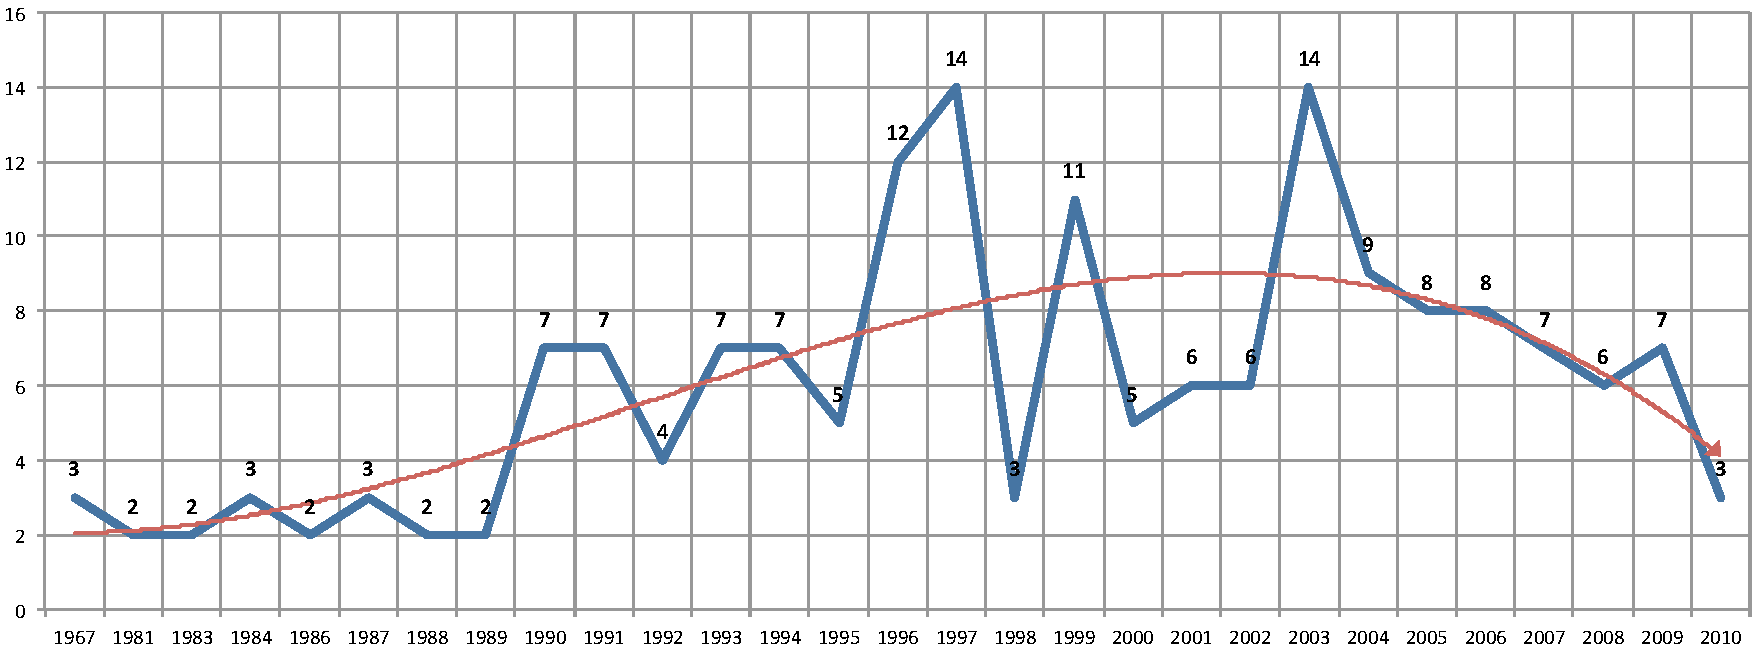
\includegraphics[scale=0.5]{imagens/abntex2-modelo-img-grafico.pdf}
	\end{center}
	\legend{Fonte: \cite[p. 24]{araujo2012}}
\end{figure}

% ---
\subsection{Figuras em \emph{minipages}}
% ---

\emph{Minipages} são usadas para inserir textos ou outros elementos em quadros
com tamanhos e posições controladas. Veja o exemplo da
\autoref{fig_minipage_imagem1} e da \autoref{fig_minipage_grafico2}.

\begin{figure}[htb]
 \label{teste}
 \centering
  \begin{minipage}{0.4\textwidth}
    \centering
    \caption{Imagem 1 da minipage} \label{fig_minipage_imagem1}
    
\includegraphics[scale=0.9]{imagens/abntex2-modelo-img-marca.pdf}
    \legend{Fonte: Produzido pelos autores}
  \end{minipage}
  \hfill
  \begin{minipage}{0.4\textwidth}
    \centering
    \caption{Grafico 2 da minipage} \label{fig_minipage_grafico2}
    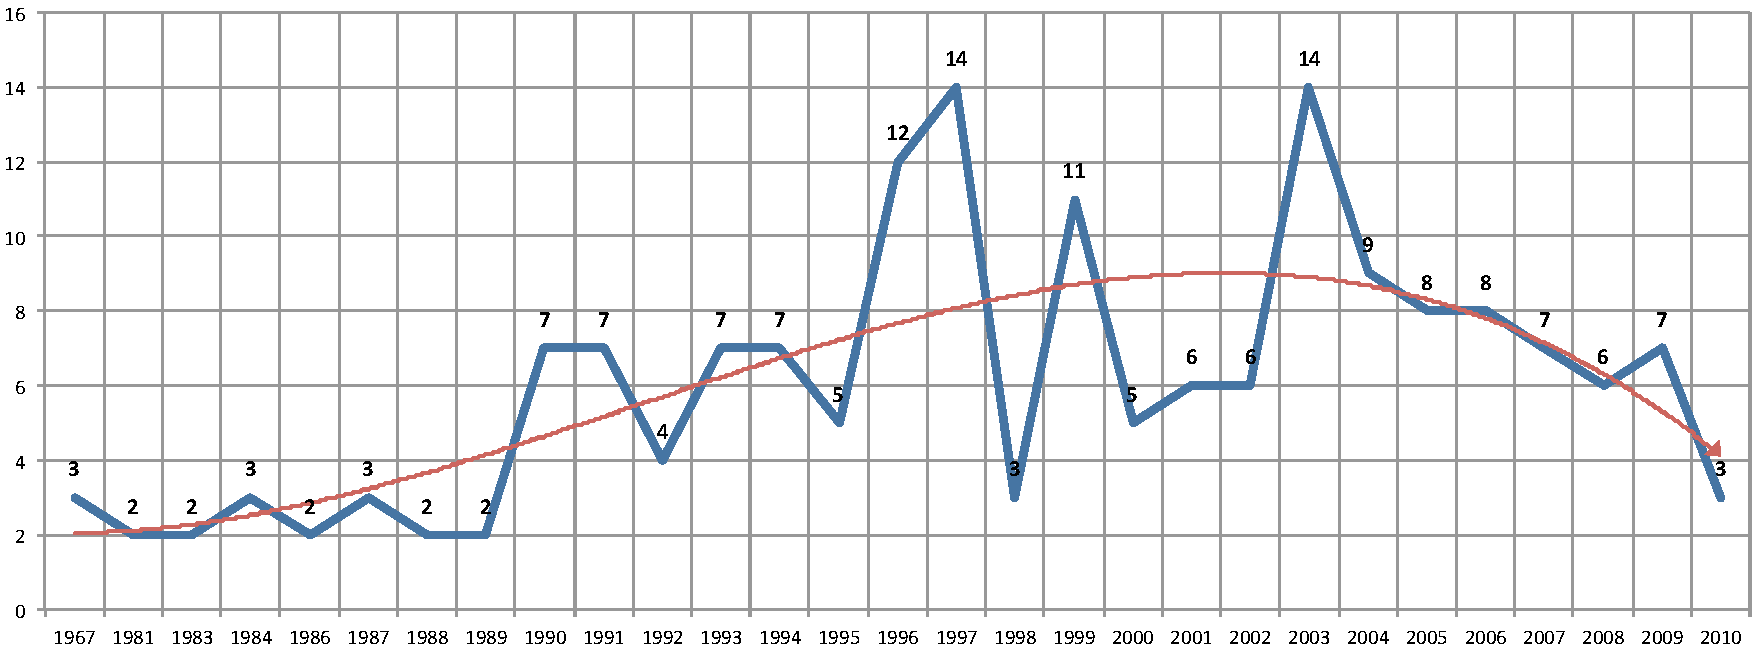
\includegraphics[scale=0.2]{imagens/abntex2-modelo-img-grafico.pdf}
    \legend{Fonte: \cite[p. 24]{araujo2012}}
  \end{minipage}
\end{figure}

Observe que, segundo a \cite[seções 4.2.1.10 e 5.8]{NBR14724:2011}, as
ilustrações devem sempre ter numeração contínua e única em todo o documento:

\begin{citacao}
Qualquer que seja o tipo de ilustração, sua identificação aparece na parte
superior, precedida da palavra designativa (desenho, esquema, fluxograma,
fotografia, gráfico, mapa, organograma, planta, quadro, retrato, figura,
imagem, entre outros), seguida de seu número de ordem de ocorrência no texto,
em algarismos arábicos, travessão e do respectivo título. Após a ilustração, na
parte inferior, indicar a fonte consultada (elemento obrigatório, mesmo que
seja produção do próprio autor), legenda, notas e outras informações
necessárias à sua compreensão (se houver). A ilustração deve ser citada no
texto e inserida o mais próximo possível do trecho a que se
refere. \cite[seções 5.8]{NBR14724:2011}
\end{citacao}

% ---
\section{Expressões matemáticas}
% ---

\index{expressões matemáticas}Use o ambiente \texttt{equation} para escrever
expressões matemáticas numeradas:

\begin{equation}
  \forall x \in X, \quad \exists \: y \leq \epsilon
\end{equation}

Escreva expressões matemáticas entre \$ e \$, como em $ \lim_{x \to \infty}
\exp(-x) = 0 $, para que fiquem na mesma linha.

Também é possível usar colchetes para indicar o início de uma expressão
matemática que não é numerada.

\[
\left|\sum_{i=1}^n a_ib_i\right|
\le
\left(\sum_{i=1}^n a_i^2\right)^{1/2}
\left(\sum_{i=1}^n b_i^2\right)^{1/2}
\]

Consulte mais informações sobre expressões matemáticas em
\url{https://github.com/abntex/abntex2/wiki/Referencias}.

% ---
\section{Enumerações: alíneas e subalíneas}
% ---

\index{alíneas}\index{subalíneas}\index{incisos}Quando for necessário enumerar
os diversos assuntos de uma seção que não possua título, esta deve ser
subdividida em alíneas \cite[4.2]{NBR6024:2012}:

\begin{alineas}

  \item os diversos assuntos que não possuam título próprio, dentro de uma mesma
  seção, devem ser subdivididos em alíneas; 
  
  \item o texto que antecede as alíneas termina em dois pontos;
  \item as alíneas devem ser indicadas alfabeticamente, em letra minúscula,
  seguida de parêntese. Utilizam-se letras dobradas, quando esgotadas as
  letras do alfabeto;

  \item as letras indicativas das alíneas devem apresentar recuo em relação à
  margem esquerda;

  \item o texto da alínea deve começar por letra minúscula e terminar em
  ponto-e-vírgula, exceto a última alínea que termina em ponto final;

  \item o texto da alínea deve terminar em dois pontos, se houver subalínea;

  \item a segunda e as seguintes linhas do texto da alínea começa sob a
  primeira letra do texto da própria alínea;
  
  \item subalíneas \cite[4.3]{NBR6024:2012} devem ser conforme as alíneas a
  seguir:

  \begin{alineas}
     \item as subalíneas devem começar por travessão seguido de espaço;

     \item as subalíneas devem apresentar recuo em relação à alínea;

     \item o texto da subalínea deve começar por letra minúscula e terminar em
     ponto-e-vírgula. A última subalínea deve terminar em ponto final, se não
     houver alínea subsequente;

     \item a segunda e as seguintes linhas do texto da subalínea começam sob a
     primeira letra do texto da própria subalínea.
  \end{alineas}
  
  \item no \abnTeX\ estão disponíveis os ambientes \texttt{incisos} e
  \texttt{subalineas}, que em suma são o mesmo que se criar outro nível de
  \texttt{alineas}, como nos exemplos à seguir:
  
  \begin{incisos}
    \item \textit{Um novo inciso em itálico};
  \end{incisos}
  
  \item Alínea em \textbf{negrito}:
  
  \begin{subalineas}
    \item \textit{Uma subalínea em itálico};
    \item \underline{\textit{Uma subalínea em itálico e sublinhado}}; 
  \end{subalineas}
  
  \item Última alínea com \emph{ênfase}.
  
\end{alineas}

% ---
\section{Espaçamento entre parágrafos e linhas}
% ---

\index{espaçamento!dos parágrafos}O tamanho do parágrafo, espaço entre a margem
e o início da frase do parágrafo, é definido por:

\begin{verbatim}
   \setlength{\parindent}{1.3cm}
\end{verbatim}

\index{espaçamento!do primeiro parágrafo}Por padrão, não há espaçamento no
primeiro parágrafo de cada início de divisão do documento
(\autoref{sec-divisoes}). Porém, você pode definir que o primeiro parágrafo
também seja indentado, como é o caso deste documento. Para isso, apenas inclua o
pacote \textsf{indentfirst} no preâmbulo do documento:

\begin{verbatim}
   \usepackage{indentfirst}      % Indenta o primeiro parágrafo de cada seção.
\end{verbatim}

\index{espaçamento!entre os parágrafos}O espaçamento entre um parágrafo e outro
pode ser controlado por meio do comando:

\begin{verbatim}
  \setlength{\parskip}{0.2cm}  % tente também \onelineskip
\end{verbatim}

\index{espaçamento!entre as linhas}O controle do espaçamento entre linhas é
definido por:

\begin{verbatim}
  \OnehalfSpacing       % espaçamento um e meio (padrão); 
  \DoubleSpacing        % espaçamento duplo
  \SingleSpacing        % espaçamento simples	
\end{verbatim}

Para isso, também estão disponíveis os ambientes:

\begin{verbatim}
  \begin{SingleSpace} ...\end{SingleSpace}
  \begin{Spacing}{hfactori} ... \end{Spacing}
  \begin{OnehalfSpace} ... \end{OnehalfSpace}
  \begin{OnehalfSpace*} ... \end{OnehalfSpace*}
  \begin{DoubleSpace} ... \end{DoubleSpace}
  \begin{DoubleSpace*} ... \end{DoubleSpace*} 
\end{verbatim}

Para mais informações, consulte \cite[p. 47-52 e 135]{memoir}.

% ---
\section{Inclusão de outros arquivos}\label{sec-include}
% ---

É uma boa prática dividir o seu documento em diversos arquivos, e não
apenas escrever tudo em um único. Esse recurso foi utilizado neste
documento. Para incluir diferentes arquivos em um arquivo principal,
de modo que cada arquivo incluído fique em uma página diferente, utilize o
comando:

\begin{verbatim}
   \include{documento-a-ser-incluido}      % sem a extensão .tex
\end{verbatim}

Para incluir documentos sem quebra de páginas, utilize:

\begin{verbatim}
   \input{documento-a-ser-incluido}      % sem a extensão .tex
\end{verbatim}

% ---
\section{Compilar o documento \LaTeX}
% ---

Geralmente os editores \LaTeX, como o
TeXlipse\footnote{\url{http://texlipse.sourceforge.net/}}, o
Texmaker\footnote{\url{http://www.xm1math.net/texmaker/}}, entre outros,
compilam os documentos automaticamente, de modo que você não precisa se
preocupar com isso.

No entanto, você pode compilar os documentos \LaTeX usando os seguintes
comandos, que devem ser digitados no \emph{Prompt de Comandos} do Windows ou no
\emph{Terminal} do Mac ou do Linux:

\begin{verbatim}
   pdflatex ARQUIVO_PRINCIPAL.tex
   bibtex ARQUIVO_PRINCIPAL.aux
   makeindex ARQUIVO_PRINCIPAL.idx 
   makeindex ARQUIVO_PRINCIPAL.nlo -s nomencl.ist -o ARQUIVO_PRINCIPAL.nls
   pdflatex ARQUIVO_PRINCIPAL.tex
   pdflatex ARQUIVO_PRINCIPAL.tex
\end{verbatim}

% ---
\section{Remissões internas}
% ---

Ao nomear a \autoref{tab-nivinv} e a \autoref{fig_circulo}, apresentamos um
exemplo de remissão interna, que também pode ser feita quando indicamos o
\autoref{cap_exemplos}, que tem o nome \emph{\nameref{cap_exemplos}}. O número
do capítulo indicado é \ref{cap_exemplos}, que se inicia à
\autopageref{cap_exemplos}\footnote{O número da página de uma remissão pode ser
obtida também assim:
\pageref{cap_exemplos}.}.
Veja a \autoref{sec-divisoes} para outros exemplos de remissões internas entre
seções, subseções e subsubseções.

O código usado para produzir o texto desta seção é:

\begin{verbatim}
Ao nomear a \autoref{tab-nivinv} e a \autoref{fig_circulo}, apresentamos um
exemplo de remissão interna, que também pode ser feita quando indicamos o
\autoref{cap_exemplos}, que tem o nome \emph{\nameref{cap_exemplos}}. O número
do capítulo indicado é \ref{cap_exemplos}, que se inicia à
\autopageref{cap_exemplos}\footnote{O número da página de uma remissão pode ser
obtida também assim:
\pageref{cap_exemplos}.}.
Veja a \autoref{sec-divisoes} para outros exemplos de remissões internas entre
seções, subseções e subsubseções.
\end{verbatim}

% ---
\section{Divisões do documento: seção}\label{sec-divisoes}
% ---

Esta seção testa o uso de divisões de documentos. Esta é a
\autoref{sec-divisoes}. Veja a \autoref{sec-divisoes-subsection}.

\subsection{Divisões do documento: subseção}\label{sec-divisoes-subsection}

Isto é uma subseção. Veja a \autoref{sec-divisoes-subsubsection}, que é uma
\texttt{subsubsection} do \LaTeX, mas é impressa chamada de ``subseção'' porque
no Português não temos a palavra ``subsubseção''.

\subsubsection{Divisões do documento: subsubseção}
\label{sec-divisoes-subsubsection}

Isto é uma subsubseção.

\subsubsection{Divisões do documento: subsubseção}

Isto é outra subsubseção.

\subsection{Divisões do documento: subseção}\label{sec-exemplo-subsec}

Isto é uma subseção.

\subsubsection{Divisões do documento: subsubseção}

Isto é mais uma subsubseção da \autoref{sec-exemplo-subsec}.


\subsubsubsection{Esta é uma subseção de quinto
nível}\label{sec-exemplo-subsubsubsection}

Esta é uma seção de quinto nível. Ela é produzida com o seguinte comando:

\begin{verbatim}
\subsubsubsection{Esta é uma subseção de quinto
nível}\label{sec-exemplo-subsubsubsection}
\end{verbatim}

\subsubsubsection{Esta é outra subseção de quinto nível}\label{sec-exemplo-subsubsubsection-outro}

Esta é outra seção de quinto nível.


\paragraph{Este é um parágrafo numerado}\label{sec-exemplo-paragrafo}

Este é um exemplo de parágrafo nomeado. Ele é produzida com o comando de
parágrafo:

\begin{verbatim}
\paragraph{Este é um parágrafo nomeado}\label{sec-exemplo-paragrafo}
\end{verbatim}

A numeração entre parágrafos numeradaos e subsubsubseções são contínuas.

\paragraph{Esta é outro parágrafo numerado}\label{sec-exemplo-paragrafo-outro}

Esta é outro parágrafo nomeado.

% ---
\section{Este é um exemplo de nome de seção longo. Ele deve estar
alinhado à esquerda e a segunda e demais linhas devem iniciar logo abaixo da
primeira palavra da primeira linha}
% ---

Isso atende à norma \cite[seções de 5.2.2 a 5.2.4]{NBR14724:2011} 
 e \cite[seções de 3.1 a 3.8]{NBR6024:2012}.

% ---
\section{Diferentes idiomas e hifenizações}
\label{sec-hifenizacao}
% ---

Para usar hifenizações de diferentes idiomas, inclua nas opções do documento o
nome dos idiomas que o seu texto contém. Por exemplo (para melhor
visualização, as opções foram quebras em diferentes linhas):

\begin{verbatim}
\documentclass[
	12pt,
	openright,
	twoside,
	a4paper,
	english,
	french,
	spanish,
	brazil
	]{abntex2}
\end{verbatim}

O idioma português-brasileiro (\texttt{brazil}) é incluído automaticamente pela
classe \textsf{abntex2}. Porém, mesmo assim a opção \texttt{brazil} deve ser
informada como a última opção da classe para que todos os pacotes reconheçam o
idioma. Vale ressaltar que a última opção de idioma é a utilizada por padrão no
documento. Desse modo, caso deseje escrever um texto em inglês que tenha
citações em português e em francês, você deveria usar o preâmbulo como abaixo:

\begin{verbatim}
\documentclass[
	12pt,
	openright,
	twoside,
	a4paper,
	french,
	brazil,
	english
	]{abntex2}
\end{verbatim}

A lista completa de idiomas suportados, bem como outras opções de hifenização,
estão disponíveis em \cite[p.~5-6]{babel}.

Exemplo de hifenização em inglês\footnote{Extraído de:
\url{http://en.wikibooks.org/wiki/LaTeX/Internationalization}}:

\begin{otherlanguage*}{english}
\textit{Text in English language. This environment switches all language-related
definitions, like the language specific names for figures, tables etc. to the other
language. The starred version of this environment typesets the main text
according to the rules of the other language, but keeps the language specific
string for ancillary things like figures, in the main language of the document.
The environment hyphenrules switches only the hyphenation patterns used; it can
also be used to disallow hyphenation by using the language name
`nohyphenation'.}
\end{otherlanguage*}

Exemplo de hifenização em francês\footnote{Extraído de:
\url{http://bigbrowser.blog.lemonde.fr/2013/02/17/tu-ne-tweeteras-point-le-vatican-interdit-aux-cardinaux-de-tweeter-pendant-le-conclave/}}:

\begin{otherlanguage*}{french}
\textit{Texte en français. Pas question que Twitter ne vienne faire une
concurrence déloyale à la traditionnelle fumée blanche qui marque l'élection
d'un nouveau pape. Pour éviter toute fuite précoce, le Vatican a donc pris un
peu d'avance, et a déjà interdit aux cardinaux qui prendront part au vote
d'utiliser le réseau social, selon Catholic News Service. Une mesure valable
surtout pour les neuf cardinaux – sur les 117 du conclave – pratiquants très
actifs de Twitter, qui auront interdiction pendant toute la période de se
connecter à leur compte.}
\end{otherlanguage*}

Pequeno texto em espanhol\footnote{Extraído de:
\url{http://internacional.elpais.com/internacional/2013/02/17/actualidad/1361102009_913423.html}}:

\foreignlanguage{spanish}{\textit{Decenas de miles de personas ovacionan al pontífice en su
penúltimo ángelus dominical, el primero desde que anunciase su renuncia. El Papa se
centra en la crítica al materialismo}}.

O idioma geral do texto por ser alterado como no exemplo seguinte:

\begin{verbatim}
  \selectlanguage{english}
\end{verbatim}

Isso altera automaticamente a hifenização e todos os nomes constantes de
referências do documento para o idioma inglês. Consulte o manual da classe
\cite{abntex2classe} para obter orientações adicionais sobre internacionalização de
documentos produzidos com \abnTeX.

A \autoref{sec-citacao} descreve o ambiente \texttt{citacao} que pode receber
como parâmetro um idioma a ser usado na citação.

% ---
\section{Consulte o manual da classe \textsf{abntex2}}
% ---

Consulte o manual da classe \textsf{abntex2} \cite{abntex2classe} para uma
referência completa das macros e ambientes disponíveis. 

Além disso, o manual possui informações adicionais sobre as normas ABNT
observadas pelo \abnTeX\ e considerações sobre eventuais requisitos específicos
não atendidos, como o caso da \cite[seção 5.2.2]{NBR14724:2011}, que
especifica o espaçamento entre os capítulos e o início do texto, regra
propositalmente não atendida pelo presente modelo.

% ---
\section{Referências bibliográficas}
% ---

A formatação das referências bibliográficas conforme as regras da ABNT são um
dos principais objetivos do \abnTeX. Consulte os manuais
\cite{abntex2cite} e \cite{abntex2cite-alf} para obter informações
sobre como utilizar as referências bibliográficas.

%-
\subsection{Acentuação de referências bibliográficas}
%-

Normalmente não há problemas em usar caracteres acentuados em arquivos
bibliográficos (\texttt{*.bib}). Porém, como as regras da ABNT fazem uso quase
abusivo da conversão para letras maiúsculas, é preciso observar o modo como se
escreve os nomes dos autores. Na ~\autoref{tabela-acentos} você encontra alguns
exemplos das conversões mais importantes. Preste atenção especial para `ç' e `í'
que devem estar envoltos em chaves. A regra geral é sempre usar a acentuação
neste modo quando houver conversão para letras maiúsculas.

\begin{table}[htbp]
\caption{Tabela de conversão de acentuação.}
\label{tabela-acentos}

\begin{center}
\begin{tabular}{ll}\hline\hline
acento & \textsf{bibtex}\\
à á ã & \verb+\`a+ \verb+\'a+ \verb+\~a+\\
í & \verb+{\'\i}+\\
ç & \verb+{\c c}+\\
\hline\hline
\end{tabular}
\end{center}
\end{table}


% ---
\section{Precisa de ajuda?}
% ---

Consulte a FAQ com perguntas frequentes e comuns no portal do \abnTeX:
\url{https://github.com/abntex/abntex2/wiki/FAQ}.

Inscreva-se no grupo de usuários \LaTeX:
\url{http://groups.google.com/group/latex-br}, tire suas dúvidas e ajude
outros usuários.

Participe também do grupo de desenvolvedores do \abnTeX:
\url{http://groups.google.com/group/abntex2} e faça sua contribuição à
ferramenta.

% ---
\section{Você pode ajudar?}
% ---

Sua contribuição é muito importante! Você pode ajudar na divulgação, no
desenvolvimento e de várias outras formas. Veja como contribuir com o \abnTeX\
em \url{https://github.com/abntex/abntex2/wiki/Como-Contribuir}.

% ---
\section{Quer customizar os modelos do \abnTeX\ para sua instituição ou
universidade?}
% ---

Veja como customizar o \abnTeX\ em:
\url{https://github.com/abntex/abntex2/wiki/ComoCustomizar}.


% ----------------------------------------------------------
% ELEMENTOS PÓS-TEXTUAIS
% ----------------------------------------------------------
\postextual
% ----------------------------------------------------------

% ----------------------------------------------------------
% Referências bibliográficas
% ----------------------------------------------------------
\bibliography{referencias}

% ----------------------------------------------------------
% Glossário
% ----------------------------------------------------------
%
% Consulte o manual da classe abntex2 para orientações sobre o glossário.
%
%\glossary

% ---
% Apêndices e Anexos
% ---
%\begin{apendicesenv}

% ----------------------------------------------------------
\chapter{Quisque libero justo}
% ----------------------------------------------------------

\lipsum[50]

% ----------------------------------------------------------
\chapter{Nullam elementum urna vel imperdiet sodales elit ipsum pharetra ligula
ac pretium ante justo a nulla curabitur tristique arcu eu metus}
% ----------------------------------------------------------
\lipsum[55-57]

\end{apendicesenv}

%\begin{anexosenv}


% ---
\chapter{Morbi ultrices rutrum lorem.}
% ---
\lipsum[30]

% ---
\chapter{Cras non urna sed feugiat cum sociis natoque penatibus et magnis dis
parturient montes nascetur ridiculus mus}
% ---

\lipsum[31]

% ---
\chapter{Fusce facilisis lacinia dui}
% ---

\lipsum[32]

\end{anexosenv}



%---------------------------------------------------------------------
% INDICE REMISSIVO
%---------------------------------------------------------------------
\phantompart
\printindex
%---------------------------------------------------------------------

\end{document}
